% =====================================================================================
%  Weather Trend Forecasting — PM Accelerator Tech Assessment (Advanced)
%  CONTENT LAYER. The layout layer (class, fonts, title page, colours) is meant to be
%  swapped in: replace everything between "LAYOUT START" and "LAYOUT END" (or \input
%  your own preamble) — section files only rely on graphicx, booktabs, hyperref, siunitx.
% =====================================================================================
% ---------------- LAYOUT START (placeholder, replace with your layout) ----------------
\documentclass[11pt,a4paper]{article}
\usepackage[margin=2.3cm]{geometry}
\usepackage[T1]{fontenc}
\usepackage[utf8]{inputenc}
\usepackage{lmodern}
\usepackage{microtype}
\usepackage{xcolor}
\usepackage[hidelinks]{hyperref}
\newcommand{\reporttitle}{Weather Trend Forecasting}
\newcommand{\reportsubtitle}{Global Weather Repository — cleaning, EDA, anomaly detection, forecasting and advanced analyses}
\newcommand{\reportauthor}{Author Name}  % TODO: set your name
\title{\reporttitle\\[0.3em]\large \reportsubtitle}
\author{\reportauthor\\PM Accelerator — Data Science Tech Assessment (Advanced)}
\date{\today}
% ---------------- LAYOUT END ----------------------------------------------------------

% packages the content needs (keep these when swapping the layout)
\usepackage{graphicx}
\usepackage{booktabs}
\usepackage{float}
\usepackage{caption}
\usepackage{subcaption}
\usepackage{amsmath}
\usepackage{textcomp}
\usepackage{gensymb}
\usepackage{newunicodechar}
\newunicodechar{°}{\textdegree}
\newunicodechar{≤}{\ensuremath{\leq}}
\newunicodechar{Δ}{\ensuremath{\Delta}}
\newunicodechar{µ}{\textmu}
\newunicodechar{³}{\textsuperscript{3}}
\newunicodechar{ü}{\"u}
\graphicspath{{../figures/}}
\usepackage{adjustbox}
\usepackage{etoolbox}
% auto-generated pandas tables: centred, small, and never wider than the text block
\AtBeginEnvironment{table}{\centering\small}
\BeforeBeginEnvironment{tabular}{\begin{adjustbox}{max width=\linewidth}}
\AfterEndEnvironment{tabular}{\end{adjustbox}}
\newcommand{\tbl}[1]{\input{../tables/#1}}

\begin{document}
\maketitle
\begin{tauenv}[frametitle=PM Accelerator — Mission]
PM Accelerator (Dr.\ Nancy Li) is a global community that helps aspiring and current product managers fast-track
their careers through coaching, an AI Product Management bootcamp and hands-on product experience. Its non-profit
arm, \emph{PMA Kids}, offers free product-management education to teenagers from underserved families:

\emph{``Our mission is to break down financial barriers and achieve educational fairness. With the goal of
establishing 200 schools worldwide over the next 20 years, we aim to empower more kids for a better future in their
life and career, simultaneously fostering a diverse landscape in the tech industry.''}

{\small Source: \url{https://www.pmaccelerator.io/}}
\end{tauenv}

\tableofcontents
\clearpage
\section{Introduction}
The \emph{Global Weather Repository} (Kaggle, \texttt{nelgiriyewithana/global-weather-repository}) publishes one
weather snapshot per day for the capital city of almost every country, with 41 columns covering temperature,
wind, pressure, precipitation, humidity, cloud, visibility, UV, six air-quality pollutants, and astronomical data.
The version analysed here (v1106) holds \textbf{170\,928 rows} from \textbf{16~May~2024 to 13~October~2026}.

The goal is to forecast future weather trends and to show both basic and advanced data-science practice.
The whole project is one reproducible pipeline. \textbf{DVC} versions the data and models and chains the stages.
\textbf{MLflow} tracks every stage, model, metric, and artefact, and holds the model registry.
The pipeline has eight stages:
\begin{enumerate}
  \item \textbf{download}: fetch the CSV from Kaggle;
  \item \textbf{clean}: validity checks, de-duplication, corrupted-batch detection, outlier capping, imputation;
  \item \textbf{features}: daily panel, lags, rolling statistics, calendar and diurnal features, time split, normalisation;
  \item \textbf{eda}: distributions, temperature and precipitation trends, correlations, decomposition;
  \item \textbf{anomaly}: Isolation Forest, LOF, temporal robust $z$-scores, batch-level detection;
  \item \textbf{train} / \textbf{train\_global}: next-day city models and multi-step global-series models;
  \item \textbf{ensemble}: mean, inverse-RMSE-weighted and stacked ensembles;
  \item \textbf{analyses}: climate, air quality, feature importance, spatial, and geographic patterns.
\end{enumerate}

\section{Data cleaning and preprocessing}\label{sec:cleaning}
Cleaning is in \nolinkurl{src/weather/data/clean.py}. Every count below is written to
\nolinkurl{reports/metrics/clean_report.json} and logged to MLflow.

\paragraph{Schema.} The seven imperial duplicates (\textdegree F, mph, inches, miles) are dropped.
The pollutant columns are renamed (\texttt{aq\_pm25}, \dots), \texttt{last\_updated} is parsed to a timestamp,
and the snapshot's \emph{local clock hour} is kept as a covariate (Section~\ref{sec:hour}).

\paragraph{Coverage and duplicates.} 71 of the 268 location strings appear on fewer than 365 days
(3\,790 rows). They are one-off or mis-named entries and are removed, which leaves \textbf{197 capitals}.
Countries reported under translated names (e.g.\ Portuguese \emph{Polônia}, plus Cyrillic and Chinese spellings) are mapped back to
the canonical name each location uses most often. Continents come from \texttt{pycountry-convert} plus a
small override table. 385 same-day duplicate snapshots are collapsed, keeping the latest one.
Some locations are \emph{geocoding homonyms} (e.g.\ ``Yaren'' in Türkiye, ``Bogot'' in Bulgaria). Their
coordinates match the listed country, so their readings are valid weather for those coordinates and they are kept.

\paragraph{Physically invalid values.} Values outside plausible surface ranges become missing.
Examples are pressure of 3\,006\,mb, wind of 2\,963\,kph, and the sentinel $-9999$ in CO and SO$_2$.

\paragraph{Corrupted batches.} For each day we take the median, across all cities, of the absolute
difference between a city's temperature and its centred 15-day rolling median. A normal day sits near 1\,\textdegree C. On
\textbf{17~August~2026} it jumps to 8.5\,\textdegree C: Riyadh reads 15.6\,\textdegree C and Bishkek
4\,\textdegree C in mid-August. That day's weather values (186 rows) are nulled and re-imputed
(Figure~\ref{fig:batch}).

\paragraph{Outliers.} Roughly symmetric variables (temperature, feels-like, wind, gust, pressure) are capped
at a per-city fence $[Q_1-3\,\mathrm{IQR},\,Q_3+3\,\mathrm{IQR}]$. Heavy-tailed variables (precipitation and the
pollutants) are capped at the global 99.9th percentile. Capping (winsorising) keeps the row and stores a
boolean flag, so these points can still be studied in Section~\ref{sec:anomaly}.
Visibility is left out of the fence because it is reported as exactly 10\,km most of the time ($\mathrm{IQR}=0$).

\paragraph{Missing values.} Within each city, gaps are filled by time interpolation (up to 3 days), then
by the city median. Categorical gaps take the city mode. The raw file has no empty cells; every missing
value comes from the checks above.

\paragraph{Normalisation.} A \texttt{StandardScaler} is fitted on the \emph{training window only} and
persisted (\nolinkurl{models/scaler.joblib}). It is applied inside the linear model's pipeline. Anomaly
detection uses a \emph{city-local} standardisation instead (Section~\ref{sec:anomaly}).

\begin{figure}[H]\centering
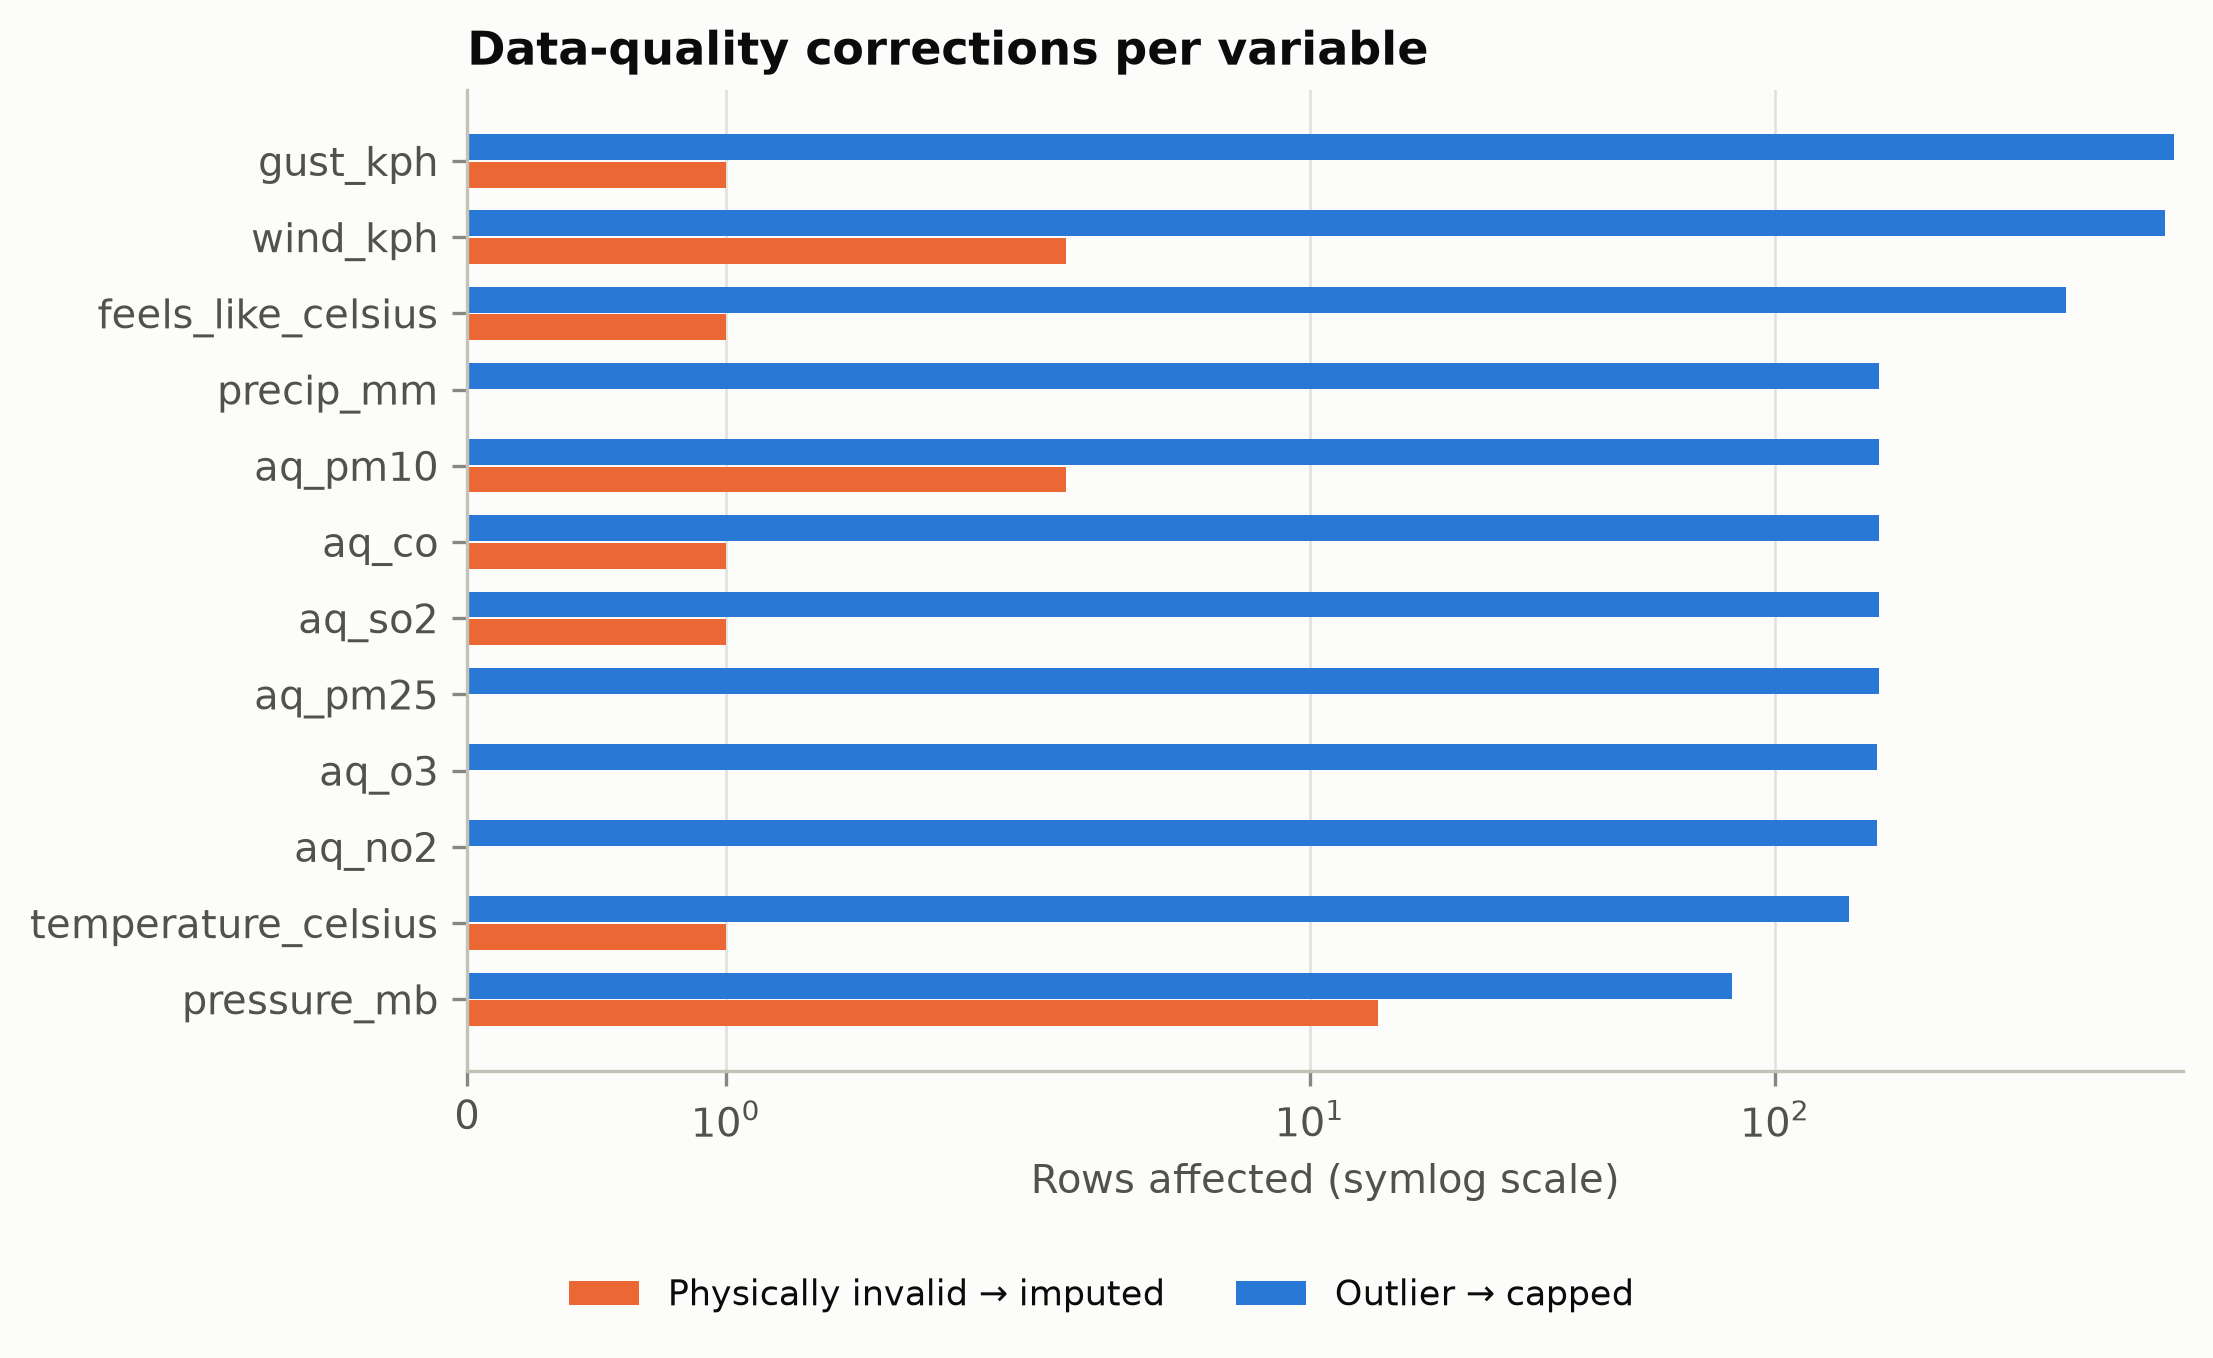
\includegraphics[width=0.75\linewidth]{eda/cleaning_corrections.png}
\caption{Rows corrected per variable: physically invalid values (imputed) and outliers (capped).}
\end{figure}

\paragraph{Feature engineering.} The cleaned data is put on a regular daily grid per city. Features use only
information available at day $t$:
\begin{itemize}
  \item today's temperature and its lags at 1, 2, 3, 7 and 14 days;
  \item rolling means and standard deviations over 3, 7 and 14 days, and the day-on-day difference;
  \item today's humidity, pressure, wind, gust, cloud, precipitation, UV, visibility and feels-like, plus
        changes in humidity and pressure;
  \item annual harmonics of the target date, also in a hemisphere-aware version;
  \item diurnal harmonics of the snapshot hour;
  \item latitude, longitude, $|$latitude$|$ and continent.
\end{itemize}
The target is temperature at $t+1$. The split is strictly by target date: the test window is the last
60 days (15~Aug--13~Oct~2026, 11\,213 rows), validation is the 60 days before it (11\,220 rows), and training is
everything earlier (142\,674 rows).

\section{Exploratory data analysis}
\tbl{summary_statistics.tex}

\subsection{Temperature}
Figure~\ref{fig:tempdist} shows that Africa and Oceania (mostly tropical capitals) are warm with narrow
distributions. Europe and Asia span more than 40\,\textdegree C over the year. The monthly curves
(Figure~\ref{fig:monthly}) show the two hemispheres in opposite phase, with Europe swinging the most.

\begin{figure}[H]\centering
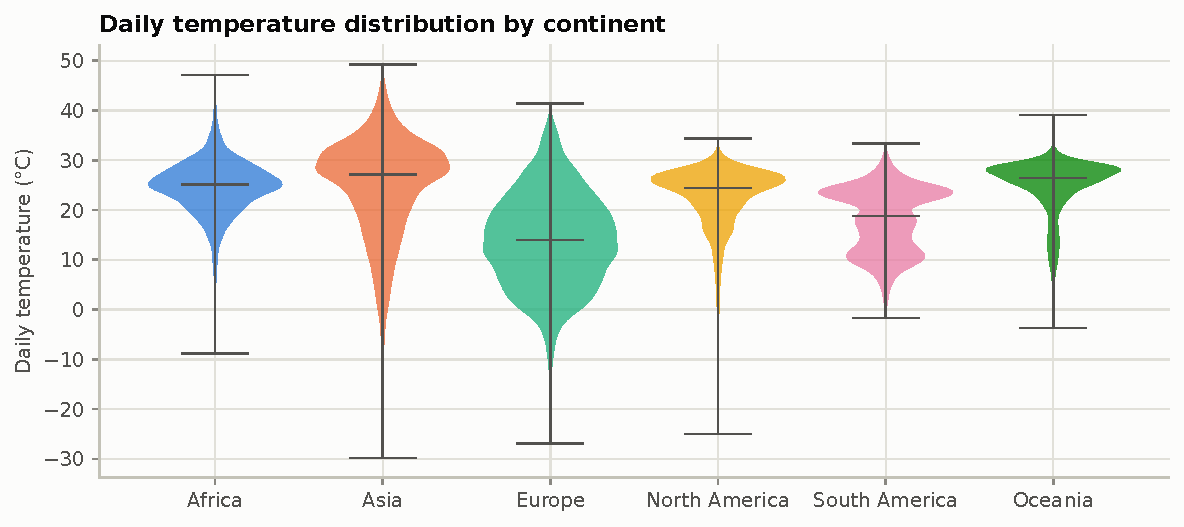
\includegraphics[width=0.85\linewidth]{eda/temperature_distribution_by_continent}
\caption{Daily temperature by continent.}\label{fig:tempdist}
\end{figure}
\begin{figure}[H]\centering
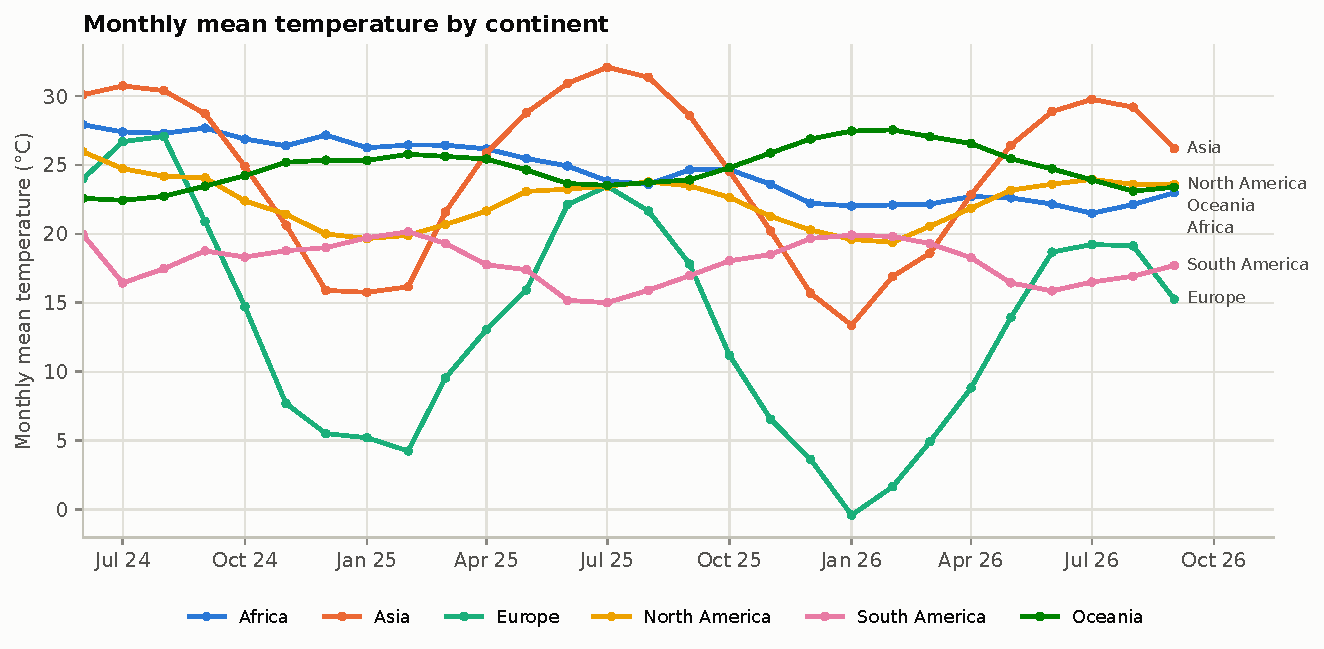
\includegraphics[width=0.9\linewidth]{eda/monthly_temperature_by_continent}
\caption{Monthly mean temperature per continent (partial first and last months removed).}\label{fig:monthly}
\end{figure}

\subsection{A hidden confounder: the snapshot hour}\label{sec:hour}
The global mean temperature of the 184 well-covered capitals (Figure~\ref{fig:global}) appears to cool
sharply. The cause is the \emph{local clock time of the snapshot}. Its median drifts from 16:30 in mid-2024
to 07:45 in late 2026 (Figure~\ref{fig:hour}), so recent observations are increasingly taken near the daily
minimum. We regress the series on a linear trend, three annual harmonics and the mean diurnal harmonics
(Figure~\ref{fig:decomp}). This shrinks the apparent trend from \textbf{$-1.80$} to
\textbf{$-0.26$\,\textdegree C/yr}, leaving an annual cycle with an amplitude of about 9.4\,\textdegree C.
Without this correction, any trend model would mistake a change in sampling for climate change.

\begin{figure}[H]\centering
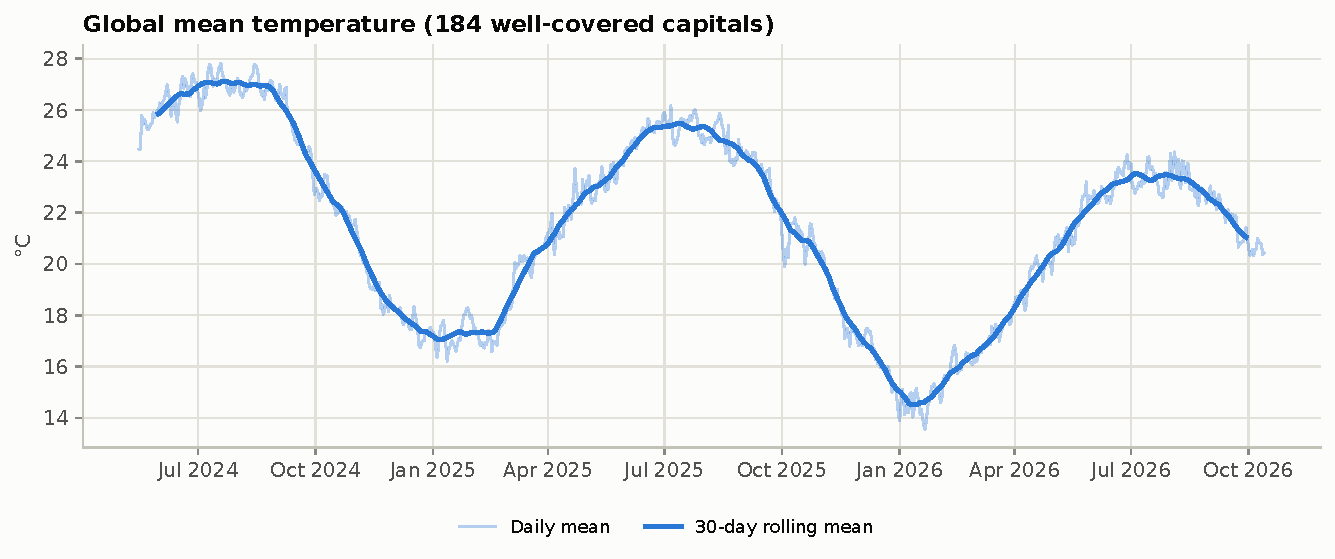
\includegraphics[width=0.9\linewidth]{eda/global_temperature_trend}
\caption{Global mean temperature, daily and 30-day rolling mean.}\label{fig:global}
\end{figure}
\begin{figure}[H]\centering
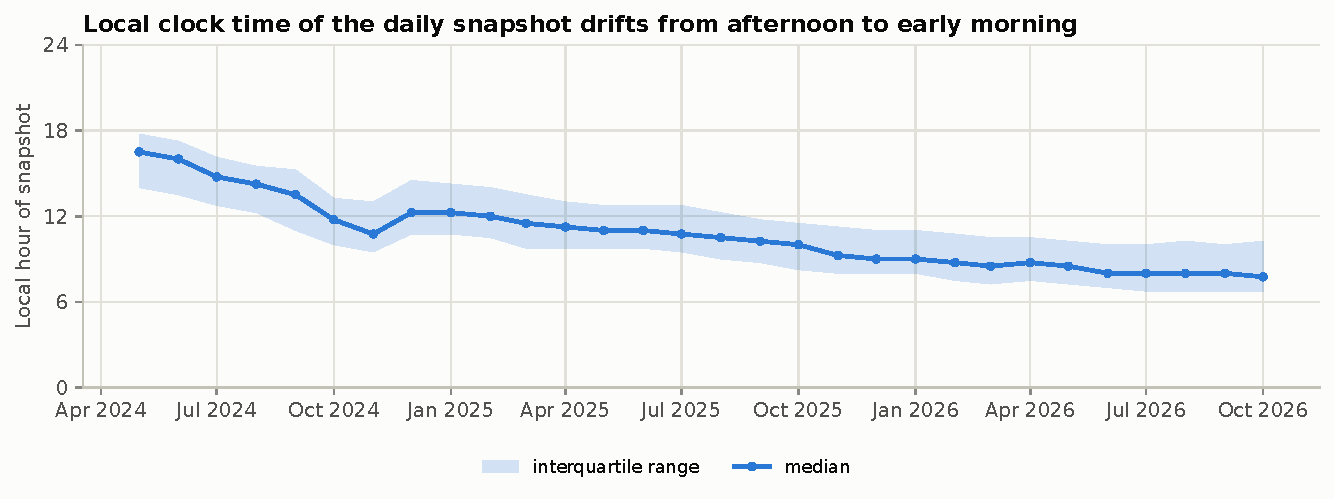
\includegraphics[width=0.9\linewidth]{eda/observation_hour_drift}
\caption{Local hour of the daily snapshot (median and IQR across cities).}\label{fig:hour}
\end{figure}
\begin{figure}[H]\centering
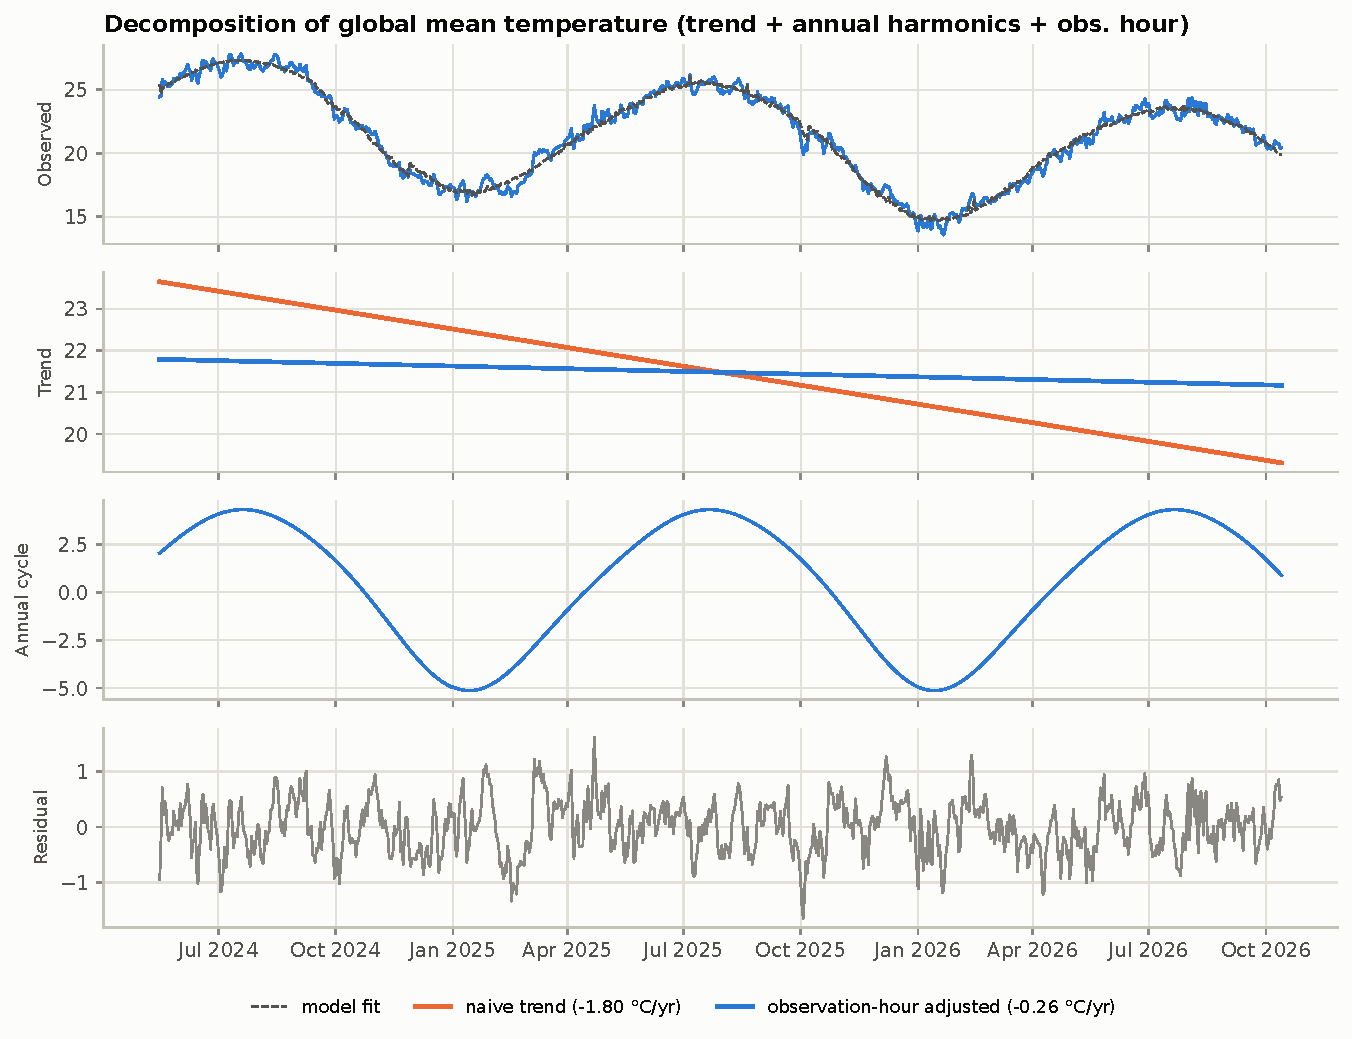
\includegraphics[width=0.9\linewidth]{eda/global_temperature_decomposition}
\caption{Harmonic-regression decomposition of global mean temperature. STL is degenerate with only about 2.4
annual cycles, so it is not used.}\label{fig:decomp}
\end{figure}

\subsection{Precipitation}
Precipitation is zero-inflated: 67\,\% of snapshots record no rain, and wet-day amounts are roughly
log-normal (Figure~\ref{fig:precip}). Seasonality differs by region (Figure~\ref{fig:precipheat}). Asia and
Oceania peak in the boreal-summer monsoon, while South America and Africa follow the migration of the ITCZ.

\begin{figure}[H]\centering
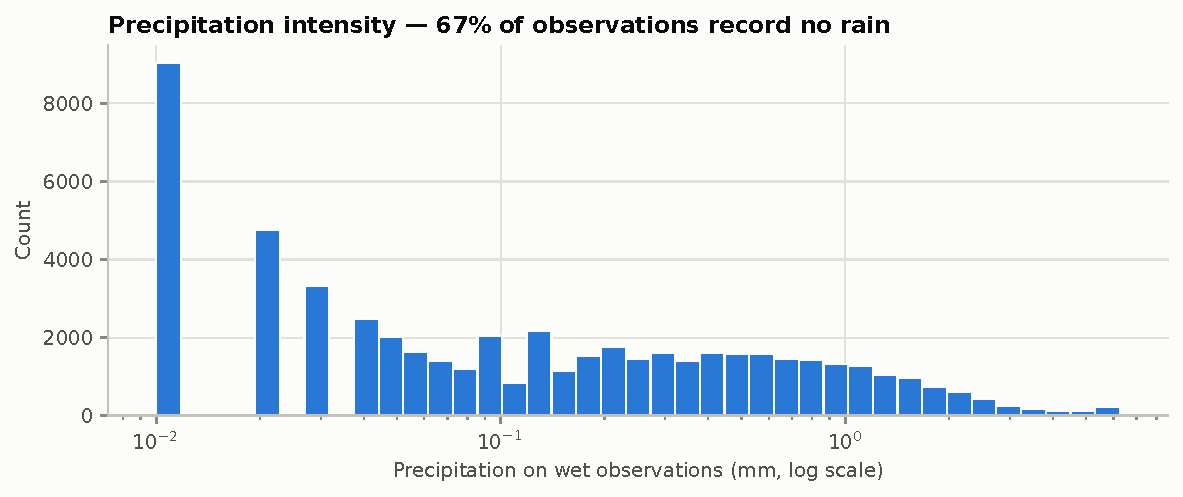
\includegraphics[width=0.8\linewidth]{eda/precipitation_distribution}
\caption{Wet-observation precipitation intensity (log scale).}\label{fig:precip}
\end{figure}
\begin{figure}[H]\centering
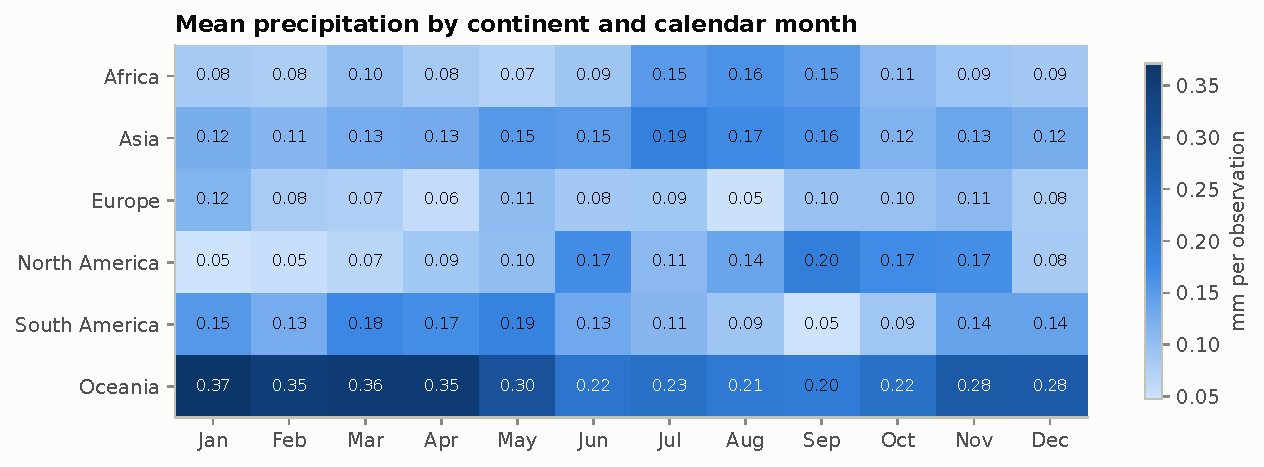
\includegraphics[width=0.9\linewidth]{eda/precipitation_heatmap_continent_month}
\caption{Mean precipitation by continent and calendar month.}\label{fig:precipheat}
\end{figure}
\begin{figure}[H]\centering
\begin{subfigure}{0.49\linewidth}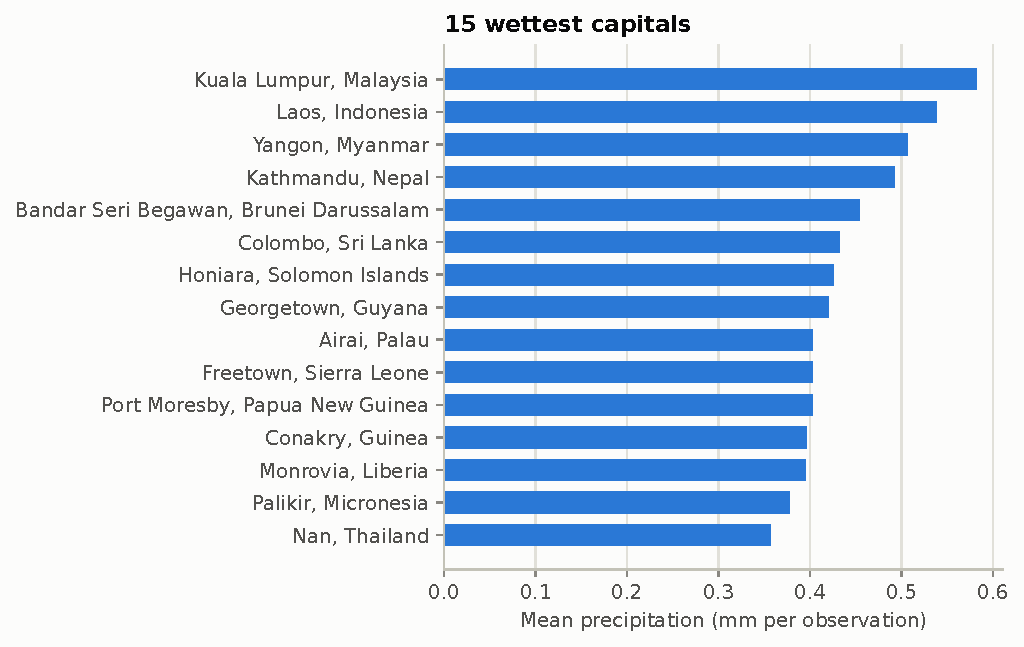
\includegraphics[width=\linewidth]{eda/wettest_capitals}\end{subfigure}
\begin{subfigure}{0.49\linewidth}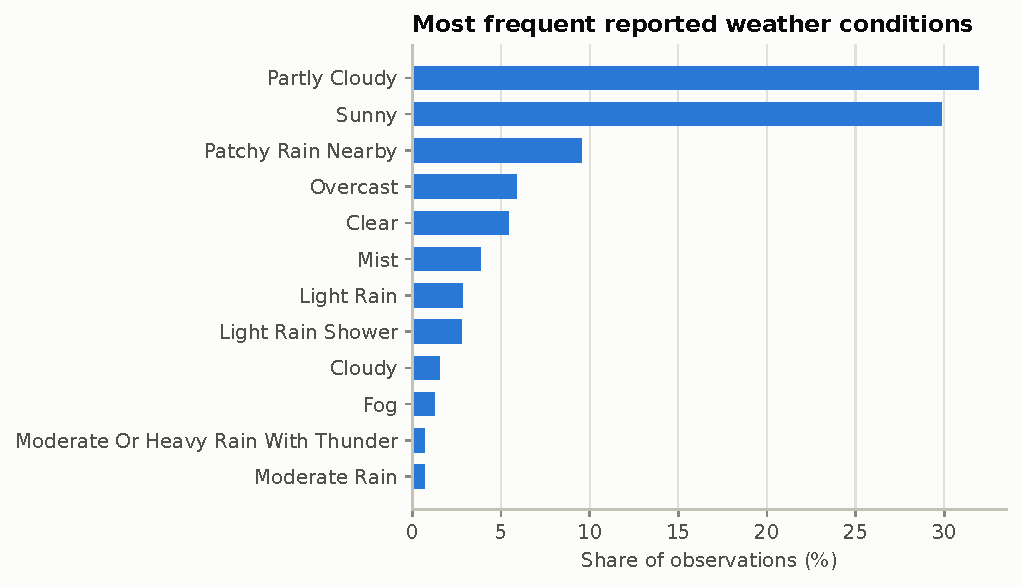
\includegraphics[width=\linewidth]{eda/weather_conditions}\end{subfigure}
\caption{Wettest capitals (left) and most frequent reported conditions (right).}
\end{figure}

\subsection{Correlations}
Spearman correlations (Figure~\ref{fig:corr}) match physical expectations:
\begin{itemize}
  \item temperature tracks feels-like and UV ($\rho\approx0.44$);
  \item humidity is anti-correlated with temperature ($\rho\approx-0.32$) and with visibility;
  \item PM2.5 and PM10 are almost collinear;
  \item ozone rises with UV and falls with humidity.
\end{itemize}

\begin{figure}[H]\centering
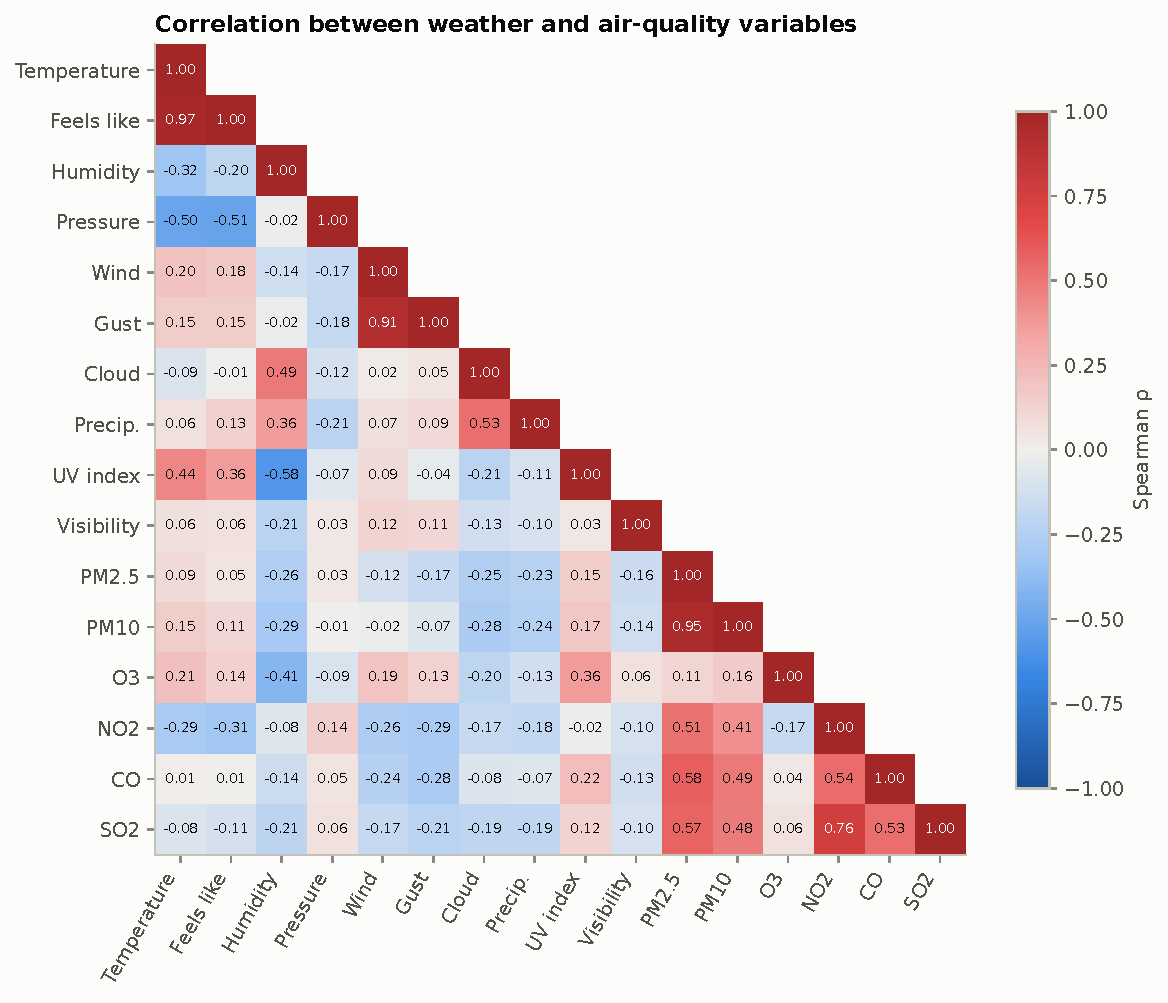
\includegraphics[width=0.72\linewidth]{eda/correlation_matrix}
\caption{Spearman correlation matrix of weather and air-quality variables.}\label{fig:corr}
\end{figure}

\section{Anomaly detection}\label{sec:anomaly}
Raw values would flag every Arctic or desert capital simply for being itself. Anomalies are therefore defined
relative to each city's own climate: temperature is standardised against the city-and-month mean, and the
other variables against the city mean. Four complementary detectors are used.
\begin{enumerate}
  \item \textbf{Isolation Forest} (300 trees, 1\,\% contamination) on ten locally standardised variables.
        It flags 1\,668 observations.
  \item \textbf{Local Outlier Factor} ($k=35$) on a 60\,000-row sample.
  \item \textbf{Temporal robust $z$-score}: temperature against a centred 15-day rolling median, scaled by the
        city's MAD, with $|z|>3.5$. This flags 2.6\,\% of observations, mostly sudden cold snaps or heat spikes.
  \item \textbf{Batch-level detector} (Figure~\ref{fig:batch}): days on which most cities deviate at once.
        This is a data-pipeline failure, not weather.
\end{enumerate}

Isolation Forest anomalies are driven mainly by extreme precipitation, low visibility and humidity
(Figure~\ref{fig:anomdrivers}): storms and fog events. Isolation Forest and LOF overlap only moderately
(Jaccard $\approx 0.11$). The global method looks for rare \emph{combinations}, while LOF finds sparse
neighbourhoods. About 18\,\% of Isolation Forest anomalies are also temporal anomalies, and about 19\,\% contain
a value capped during cleaning. The multivariate view therefore adds information beyond univariate fences.

\begin{figure}[H]\centering
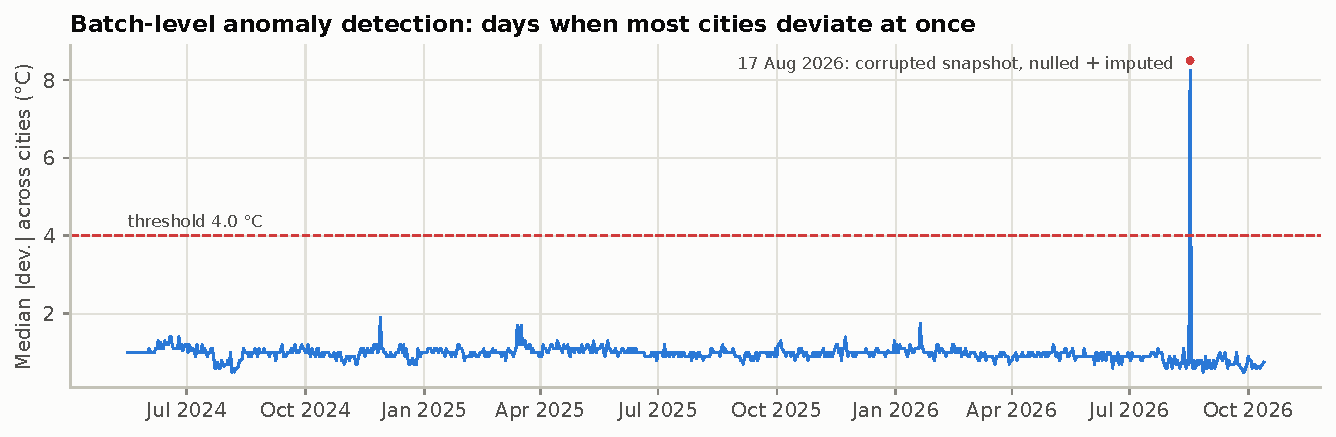
\includegraphics[width=0.9\linewidth]{anomaly/batch_corruption_detector}
\caption{Batch-level detector: the 17~Aug~2026 snapshot is corrupted and was nulled and imputed during cleaning.}\label{fig:batch}
\end{figure}
\begin{figure}[H]\centering
\begin{subfigure}{0.49\linewidth}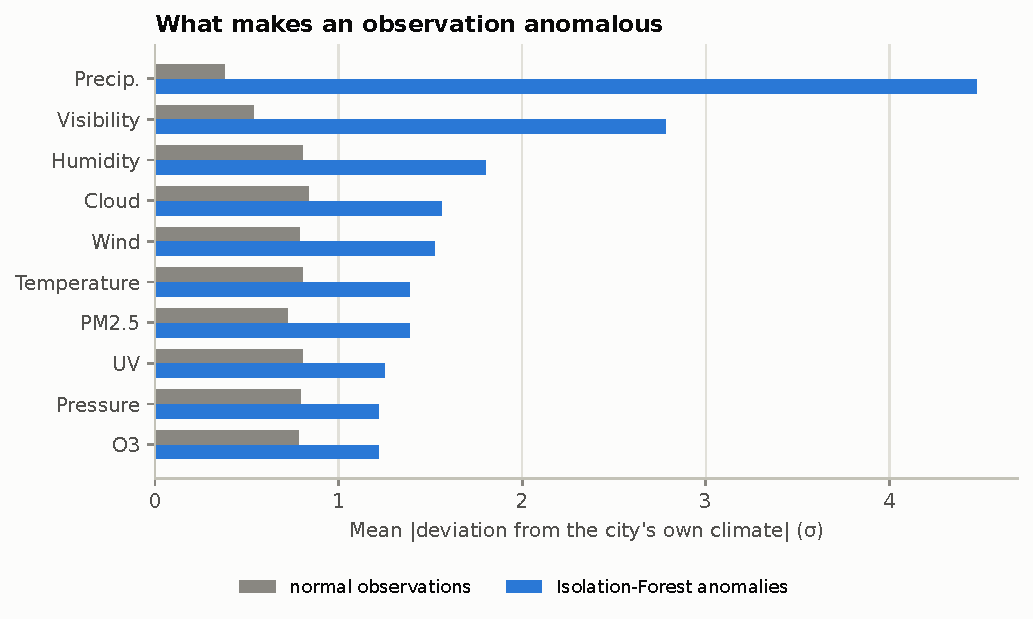
\includegraphics[width=\linewidth]{anomaly/anomaly_drivers}\caption{Drivers}\label{fig:anomdrivers}\end{subfigure}
\begin{subfigure}{0.49\linewidth}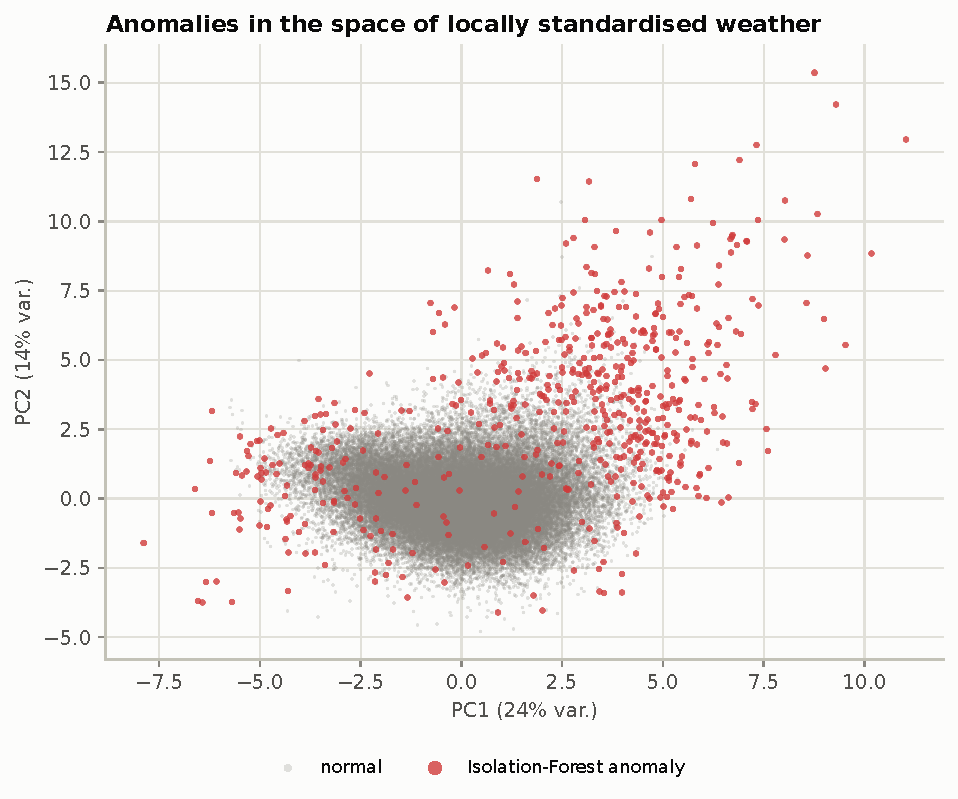
\includegraphics[width=\linewidth]{anomaly/anomaly_pca}\caption{PCA projection}\end{subfigure}
\caption{What makes an observation anomalous, and where anomalies sit in the locally standardised weather space.}
\end{figure}
\begin{figure}[H]\centering
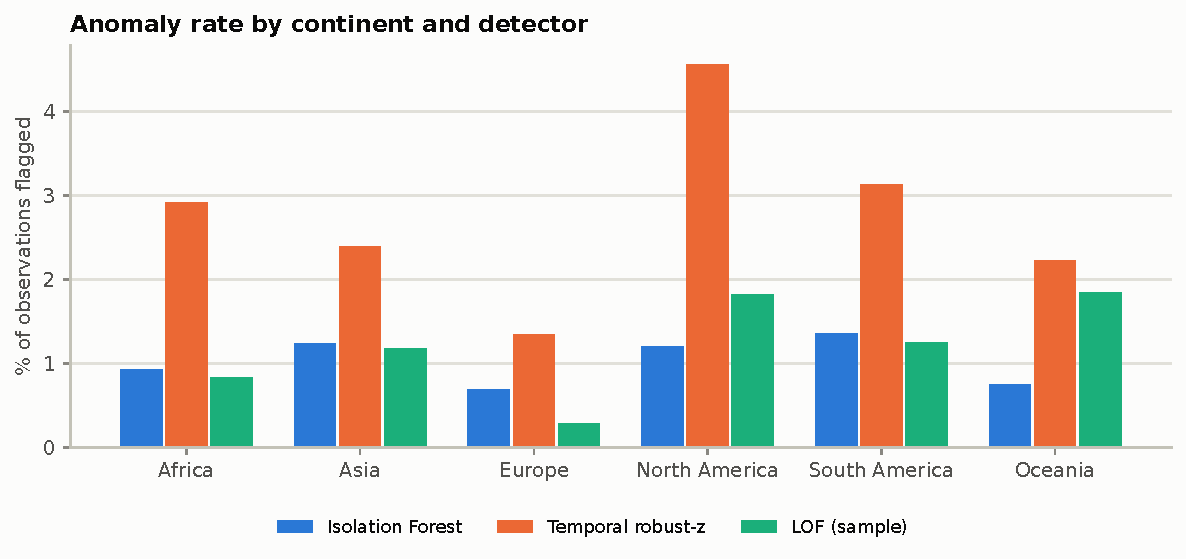
\includegraphics[width=0.85\linewidth]{anomaly/anomaly_rate_by_continent}
\caption{Anomaly rate by continent and detector.}
\end{figure}
\begin{figure}[H]\centering
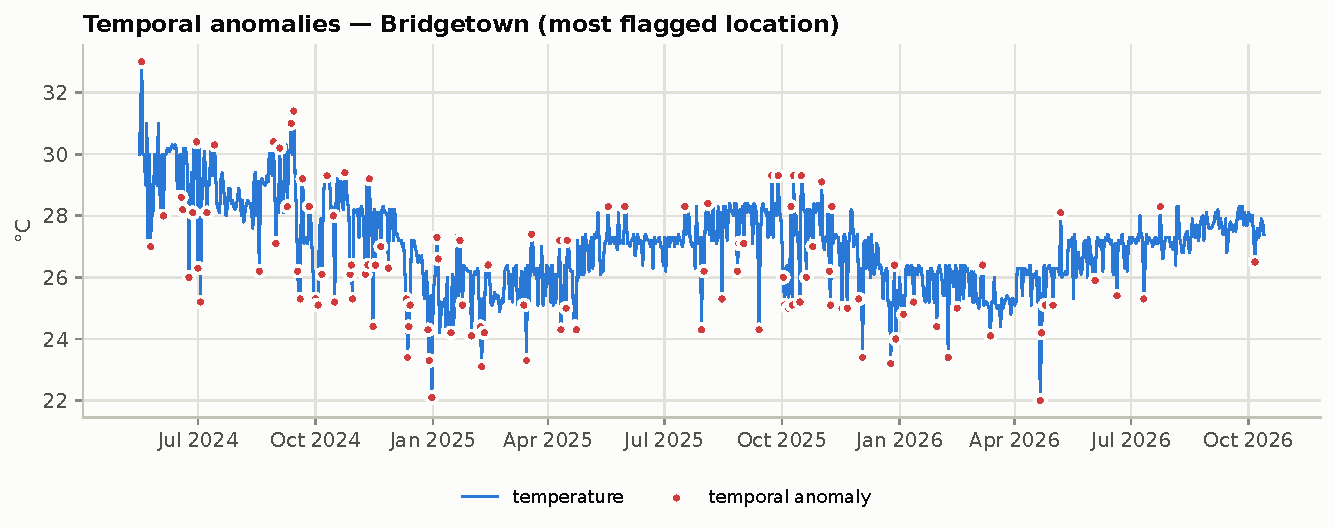
\includegraphics[width=0.9\linewidth]{anomaly/city_temporal_anomalies}
\caption{Temporal anomalies for the most-flagged capital.}
\end{figure}
\begin{figure}[H]\centering
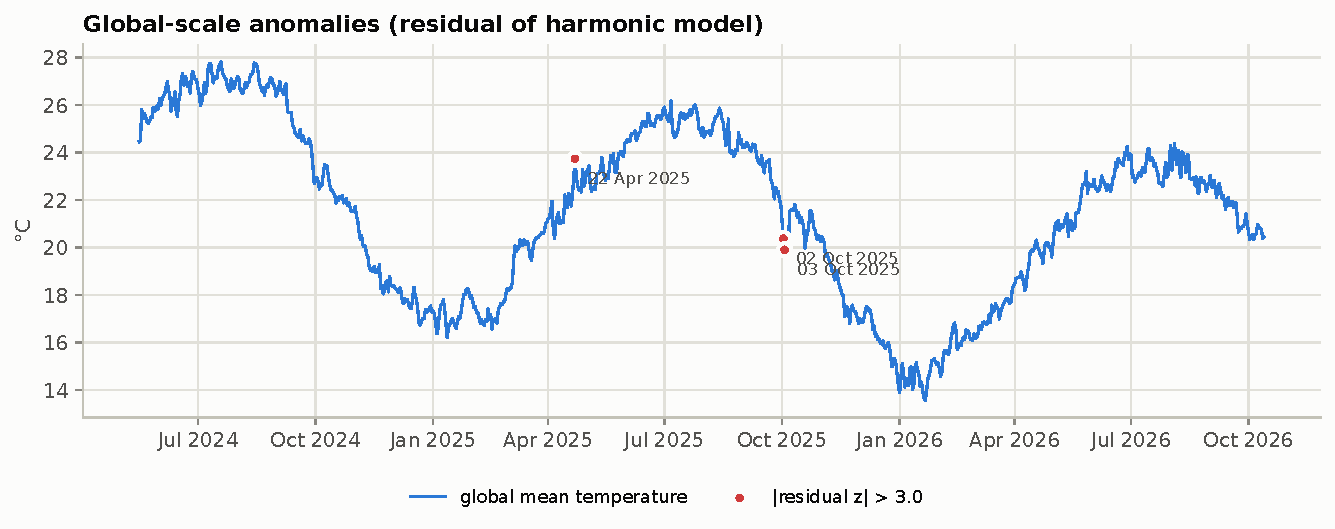
\includegraphics[width=0.9\linewidth]{anomaly/global_anomalies}
\caption{Remaining global-scale anomalies after cleaning ($|z|>3$ on the residual of the harmonic model).}
\end{figure}
\tbl{top_anomalies.tex}

\section{Forecasting}
Two framings use the \texttt{last\_updated} time axis.
\begin{itemize}
  \item \textbf{City panel, next-day forecast}: one global model learns from all 197 capitals at once.
  \item \textbf{Global mean series, 60-day multi-step forecast}: the worldwide trend is projected forward.
\end{itemize}
Every model is a nested MLflow run with its parameters, validation and test metrics, a residual plot, the
model artefact and an input signature. Each one is also registered in the MLflow Model Registry
(\texttt{weather-temp-<model>}).

\paragraph{Metrics.} MAE, RMSE, sMAPE, $R^2$, and the share of forecasts within 2\,\textdegree C.
MAPE is computed only where $|y|\ge1$\,\textdegree C, because it explodes near 0\,\textdegree C. We also
report \emph{skill}, the RMSE reduction relative to persistence (tomorrow = today).

\subsection{City panel: single models and ensembles}
Four learners are compared against persistence:
\begin{itemize}
  \item ridge regression on the train-fitted standardisation;
  \item random forest;
  \item XGBoost and LightGBM, both with early stopping on the validation window.
\end{itemize}
Three ensembles are built from validation-window predictions only:
\begin{itemize}
  \item a simple mean;
  \item an inverse-validation-RMSE weighted mean;
  \item \textbf{stacking} with non-negative least squares. Its weights are XGBoost 0.49, LightGBM 0.26,
        Ridge 0.24 and random forest 0.01.
\end{itemize}
The stacked ensemble is logged as an MLflow \texttt{pyfunc} model (\texttt{weather-temp-ensemble}). The
pipeline checks that the served model reproduces the offline predictions.

\tbl{model_comparison.tex}

All learned models beat persistence. The ensembles beat every single model, and stacking is best:
test RMSE 1.838\,\textdegree C, MAE 1.21\,\textdegree C, $R^2=0.929$, 81\,\% of forecasts within 2\,\textdegree C,
and 12.2\,\% skill. Ridge receives a meaningful weight despite being the weakest member because its errors
are the least correlated with the tree models'. The gains look modest because day-to-day weather from a single
daily snapshot is noisy; the hardest regions are mid-latitude Europe and Asia, where synoptic systems pass
through (Figure~\ref{fig:rmsecont}).

\begin{figure}[H]\centering
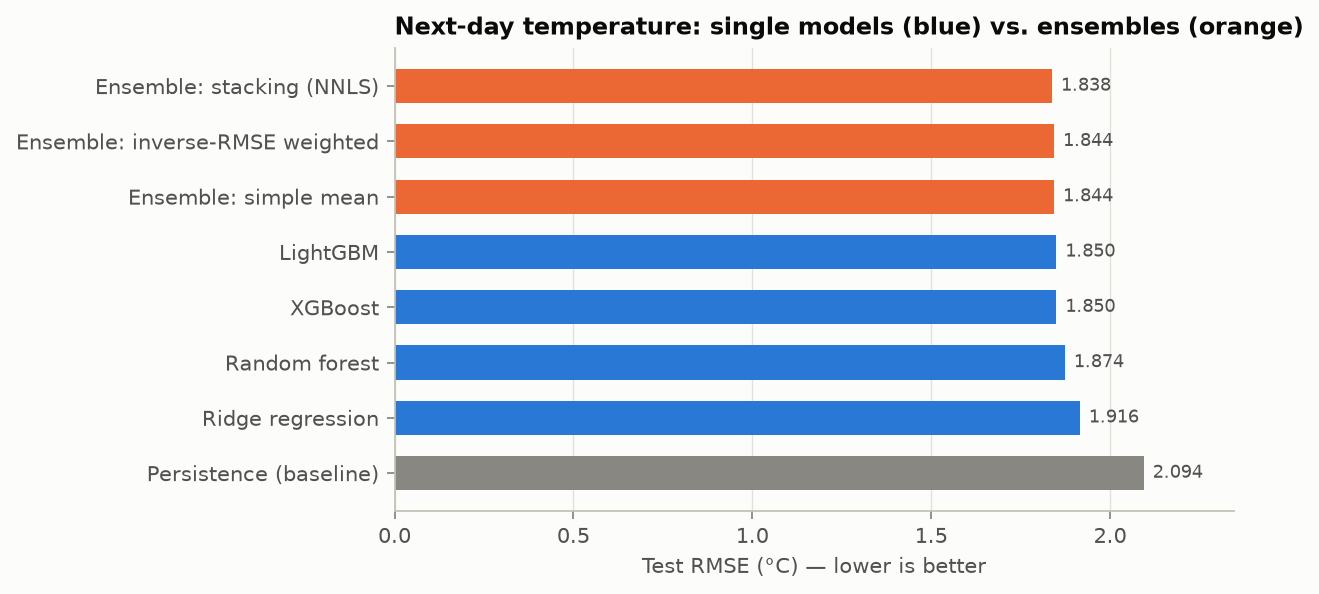
\includegraphics[width=0.85\linewidth]{forecast_panel/model_comparison_rmse.png}
\caption{Test RMSE of single models (blue) and ensembles (orange).}
\end{figure}
\begin{figure}[H]\centering
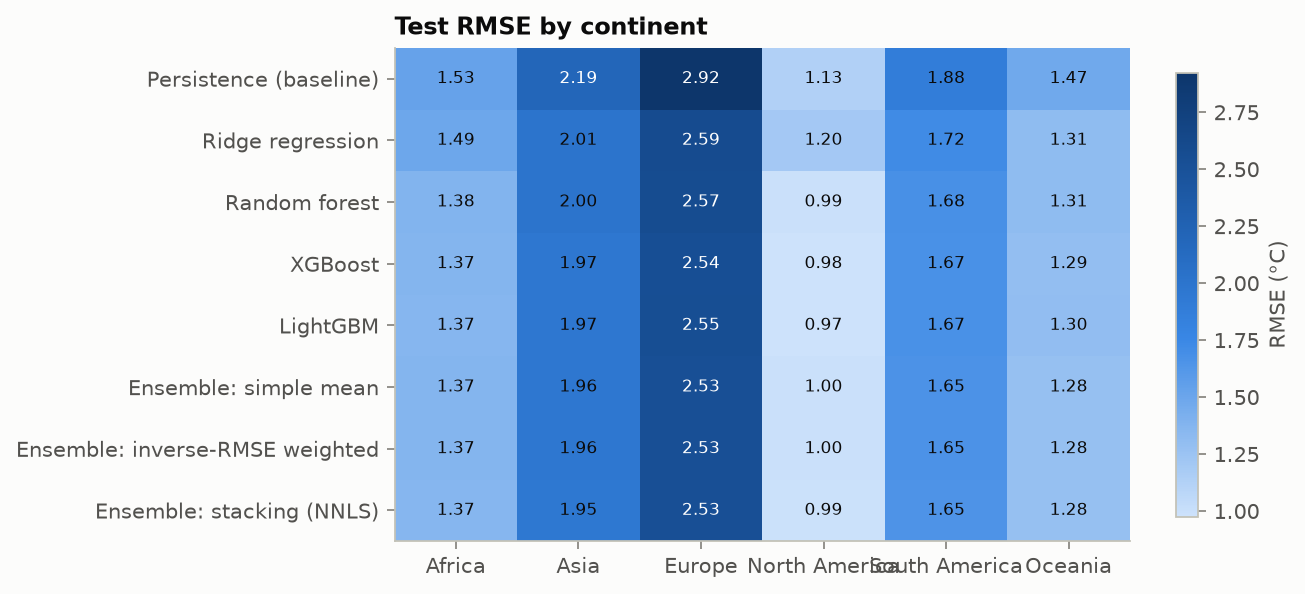
\includegraphics[width=0.85\linewidth]{forecast_panel/rmse_by_continent.png}
\caption{Test RMSE by continent.}\label{fig:rmsecont}
\end{figure}
\begin{figure}[H]\centering
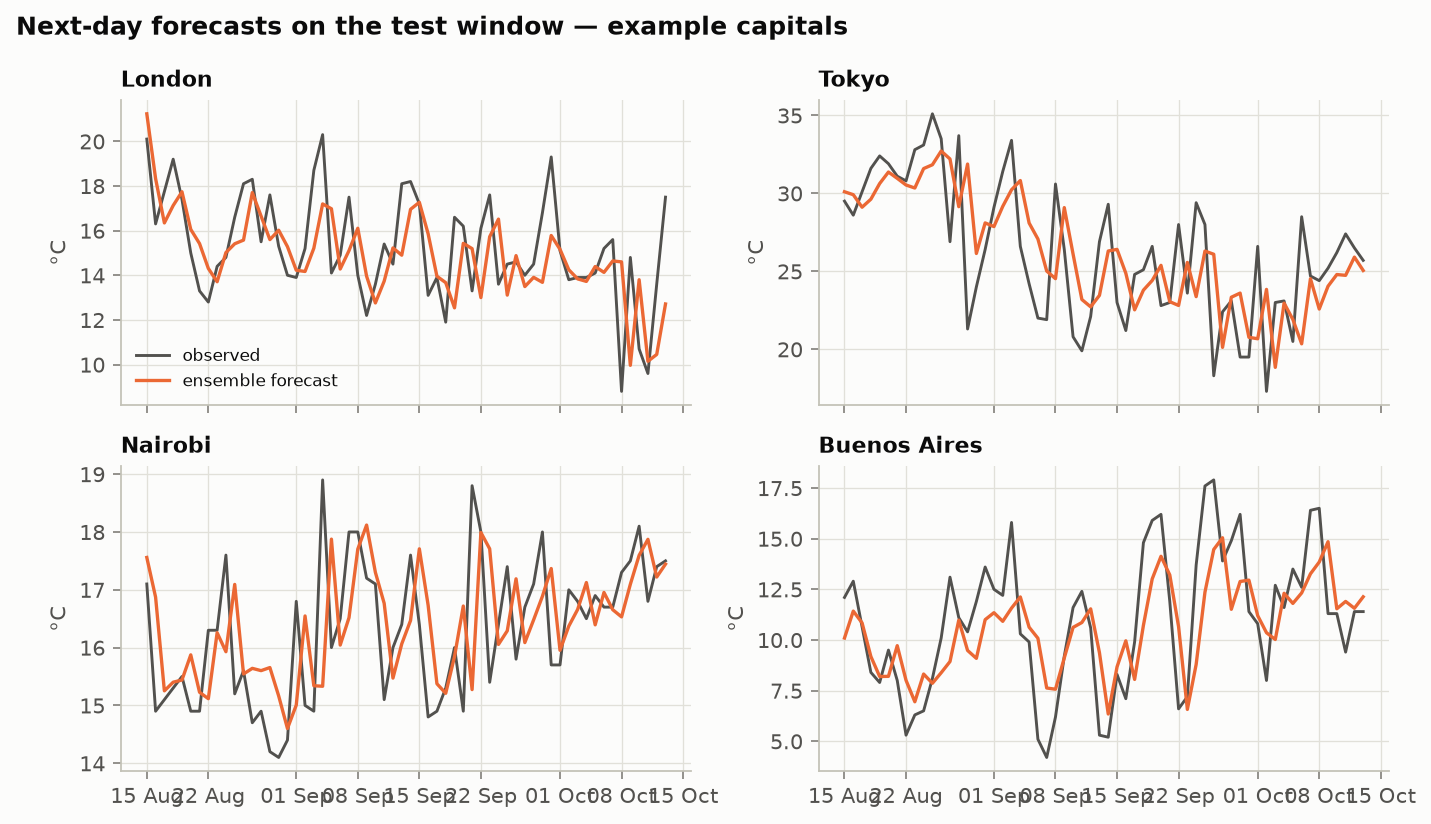
\includegraphics[width=0.9\linewidth]{forecast_panel/city_forecasts.png}
\caption{Stacked-ensemble next-day forecasts against observations for four example capitals.}
\end{figure}
\begin{figure}[H]\centering
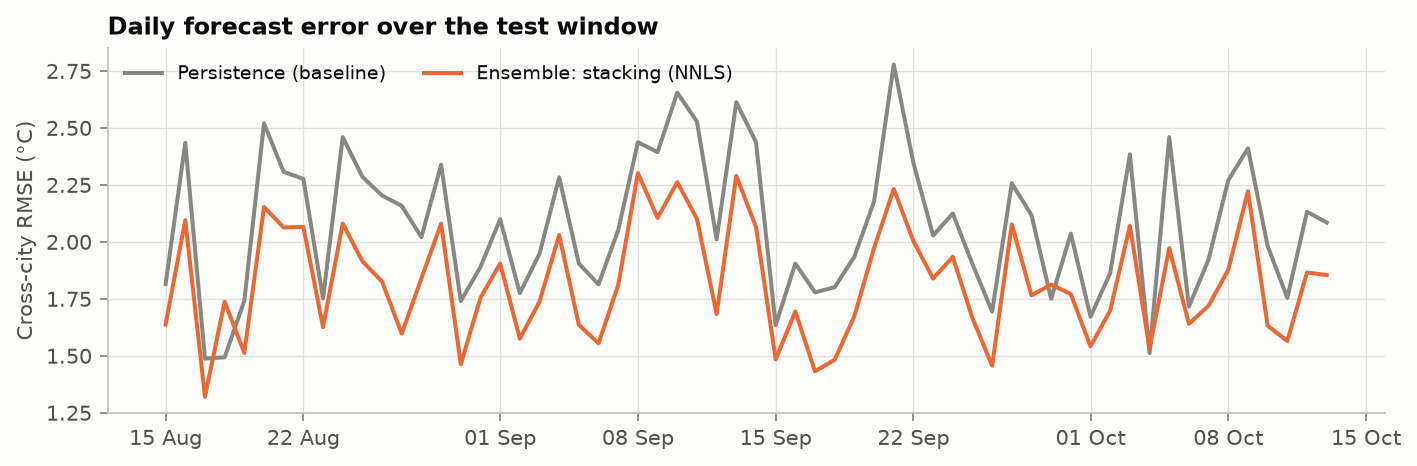
\includegraphics[width=0.9\linewidth]{forecast_panel/daily_error_test.png}
\caption{Cross-city RMSE per day over the test window.}
\end{figure}

\subsection{Global mean series: multi-step trend forecasting}
Each model is fitted on everything before the test window and forecasts all 60 test days in one shot:
\begin{itemize}
  \item naive and seasonal-naive (value 365 days earlier) baselines;
  \item damped Holt--Winters with a 365-day season;
  \item harmonic regression (trend, four annual harmonics, observation-hour harmonics);
  \item regression with ARIMA(1,0,1) errors on the same design (\texttt{sarimax\_fourier});
  \item their mean ensemble.
\end{itemize}
The snapshot hour of future days is unknown, so it is held at its last 30-day average.

\tbl{global_model_comparison.tex}

Harmonic regression and SARIMAX reach about 0.35\,\textdegree C RMSE over a 60-day horizon, four times
better than seasonal-naive. The ensemble is marginally best. Including the observation-hour terms cuts the
SARIMAX error from 0.62 to 0.37\,\textdegree C, which confirms that the confounder matters for forecasting
as well as for trend estimation. Refitted on all data, the best interval-producing model projects the next
90 days with a 95\,\% prediction interval (Figure~\ref{fig:future}).

\begin{figure}[H]\centering
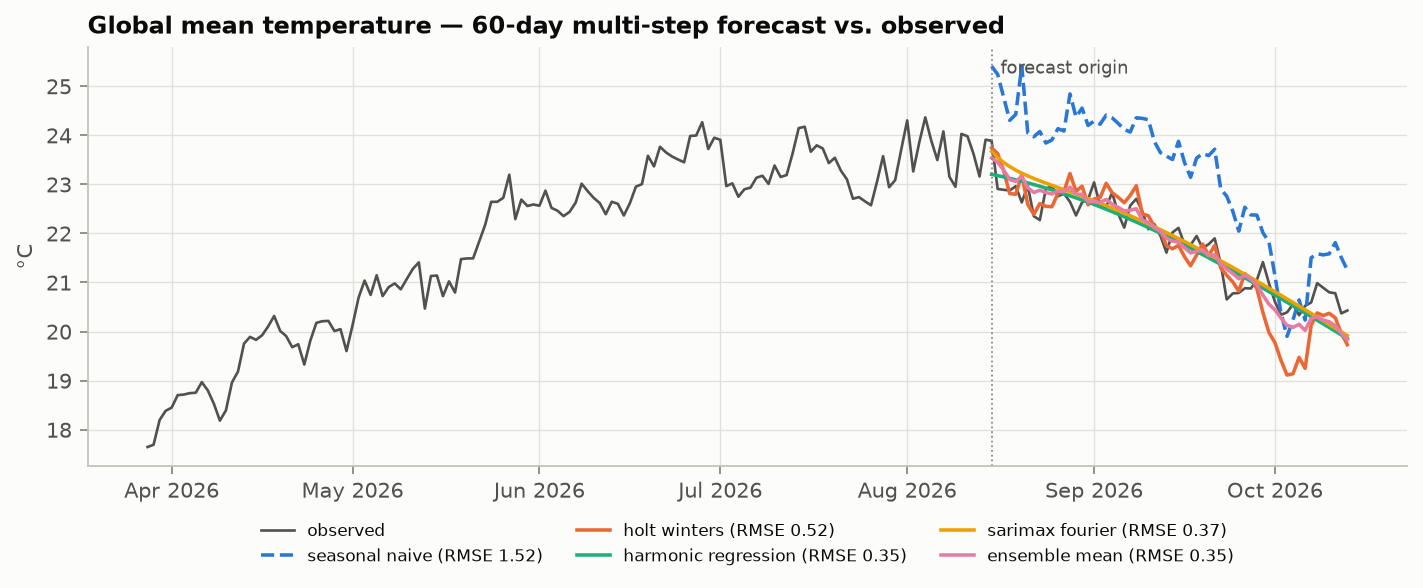
\includegraphics[width=0.9\linewidth]{forecast_global/global_multistep_forecast.png}
\caption{60-day multi-step forecasts of the global mean temperature.}
\end{figure}
\begin{figure}[H]\centering
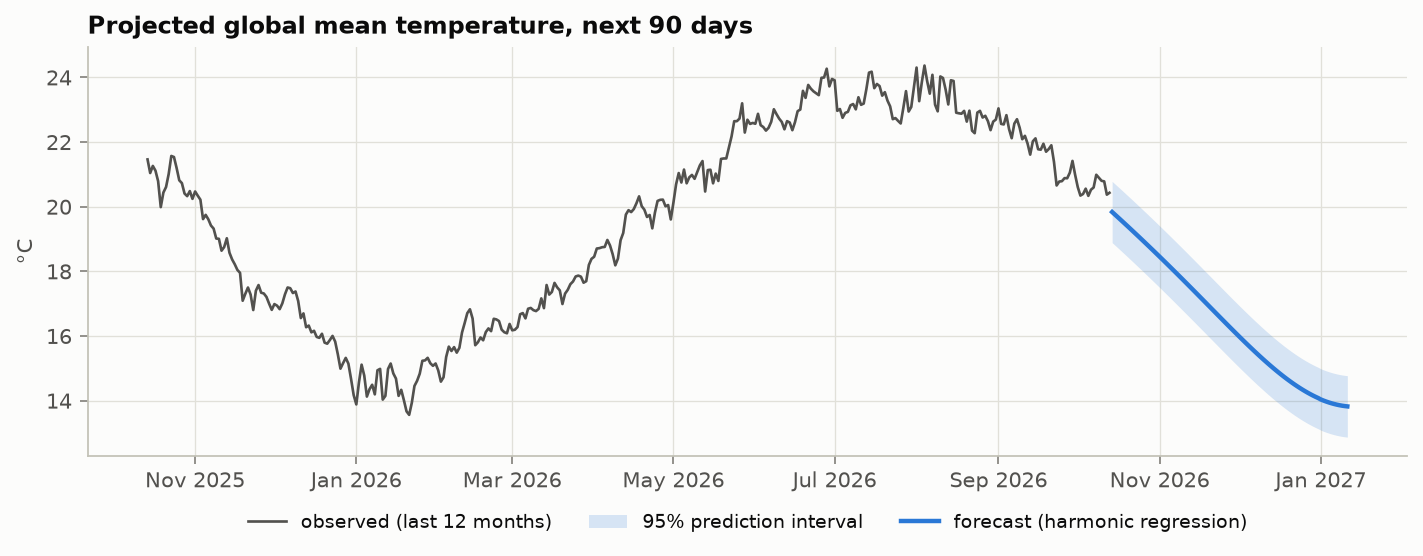
\includegraphics[width=0.9\linewidth]{forecast_global/global_future_forecast.png}
\caption{Projected global mean temperature for the next 90 days.}\label{fig:future}
\end{figure}

\section{Advanced analyses}

\subsection{Climate analysis}
For every city we fit temperature on a linear trend, two annual harmonics, and two diurnal harmonics of the
snapshot hour. The record covers only about 2.4 years, so these slopes describe short-term variation, not
climate change. Without the hour terms, 79\,\% of cities appear to cool, at a median of $-1.79$\,\textdegree C/yr.
With them the median slope falls to $-0.51$\,\textdegree C/yr (Figure~\ref{fig:climtrend}). The diurnal effect
captured by the hour terms is large: about 8\,\textdegree C peak-to-peak in the median city.
Seasonality is structured by latitude. The two hemispheres run in opposite phase
(Figure~\ref{fig:latband}), and the annual range grows strongly with $|$latitude$|$ ($r=0.84$). Continental
capitals such as Ulaanbaatar, Astana and Bishkek have the widest swings (30--42\,\textdegree C) (Figure~\ref{fig:amp}).

\begin{figure}[H]\centering
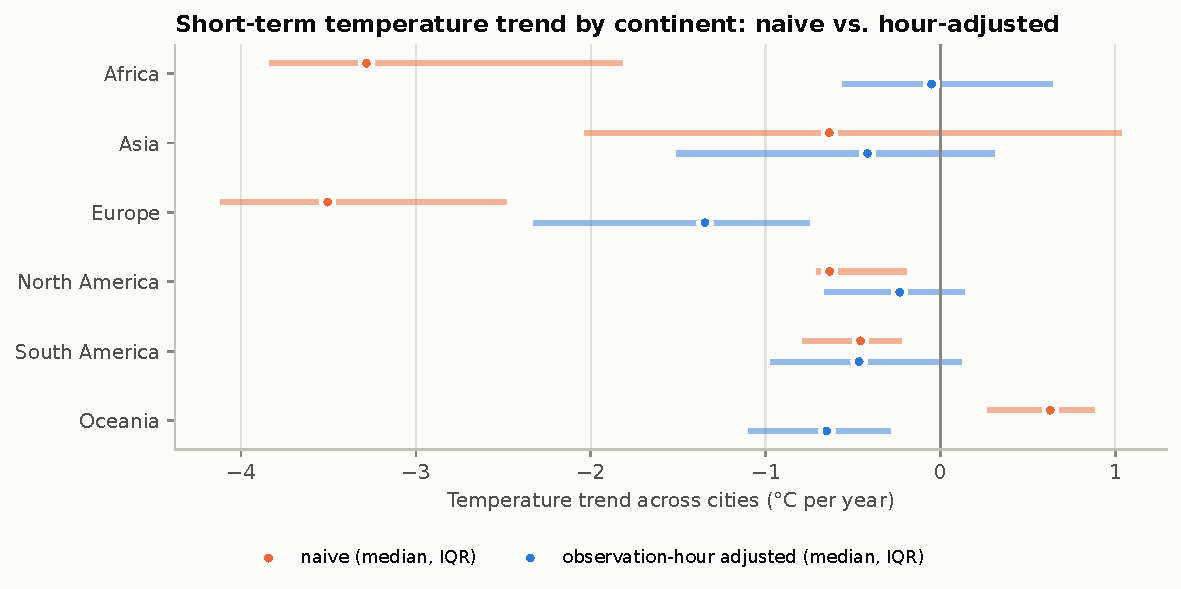
\includegraphics[width=0.85\linewidth]{analyses/climate_trend_by_continent}
\caption{Per-city temperature trends by continent, naive and observation-hour adjusted.}\label{fig:climtrend}
\end{figure}
\begin{figure}[H]\centering
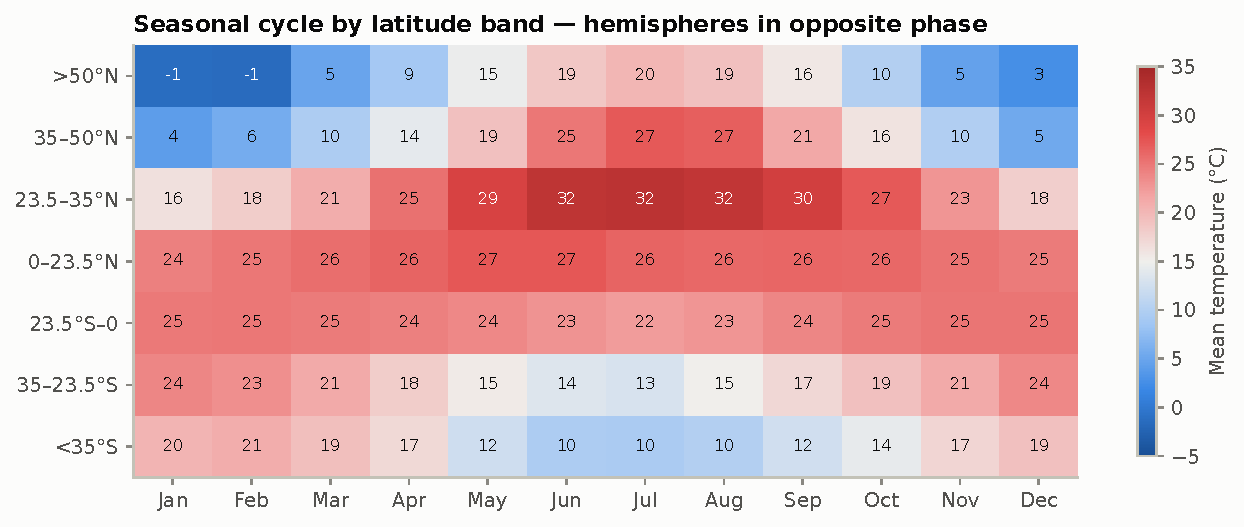
\includegraphics[width=0.9\linewidth]{analyses/climate_latitude_band_seasonality}
\caption{Mean temperature by latitude band and calendar month.}\label{fig:latband}
\end{figure}
\begin{figure}[H]\centering
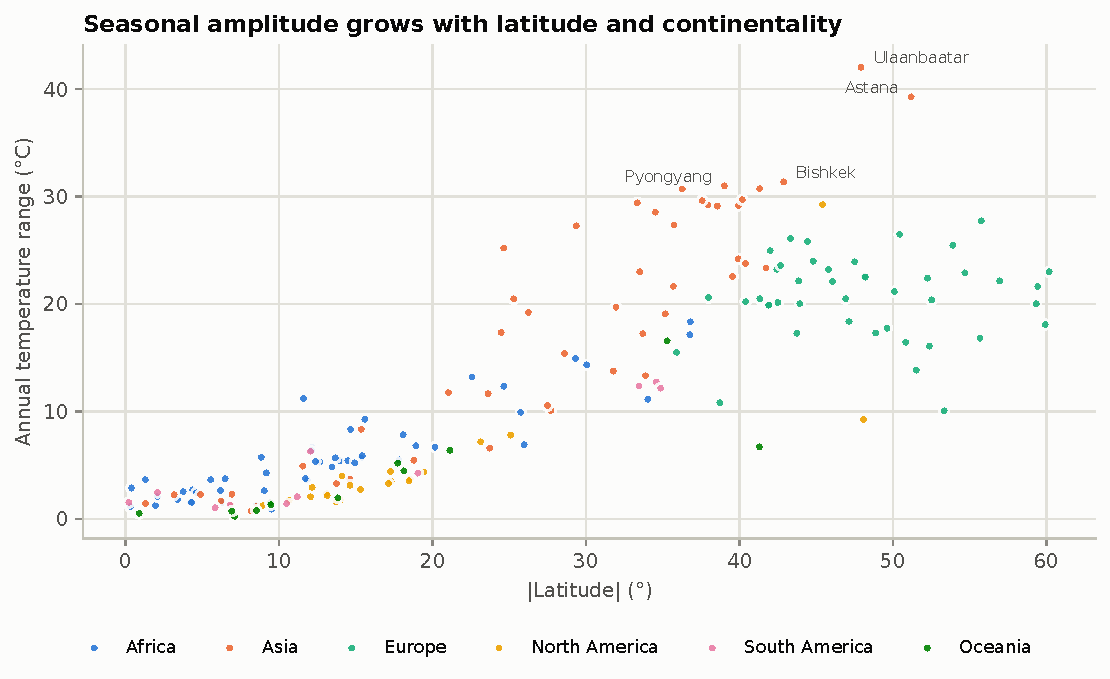
\includegraphics[width=0.75\linewidth]{analyses/climate_amplitude_vs_latitude}
\caption{Annual temperature range against $|$latitude$|$.}\label{fig:amp}
\end{figure}

\subsection{Environmental impact: air quality and weather}
Pooled correlations mix geography with weather: humid tropical capitals are cleaner than dry, dense ones.
To isolate the weather effect we also compute \emph{within-city} correlations, after removing each city's mean
(Figure~\ref{fig:aqcorr}).
\begin{itemize}
  \item \textbf{Ozone} is photochemical. It rises with temperature ($\rho=0.31$) and UV ($\rho=0.32$) and
        falls with humidity.
  \item \textbf{NO$_2$} and \textbf{SO$_2$} fall with wind (dispersion) and rise with pressure (stagnant
        anticyclones).
  \item \textbf{PM2.5} falls with wind, precipitation and cloud (wash-out and mixing). Within a city these
        effects are weak ($|\rho|\le0.13$), so particulate levels are driven mostly by local emissions.
\end{itemize}
A LightGBM model of $\log$\,PM2.5 reaches test $R^2\approx0.51$. Location (longitude and latitude) dominates
its permutation importance, calendar month barely matters, and UV, temperature and humidity are the main weather
drivers (Figure~\ref{fig:pmdrivers}). The median
PM2.5 of 41\,\% of capitals exceeds the WHO 24-hour guideline of 15\,µg/m³. Asia carries the heaviest burden.

\begin{figure}[H]\centering
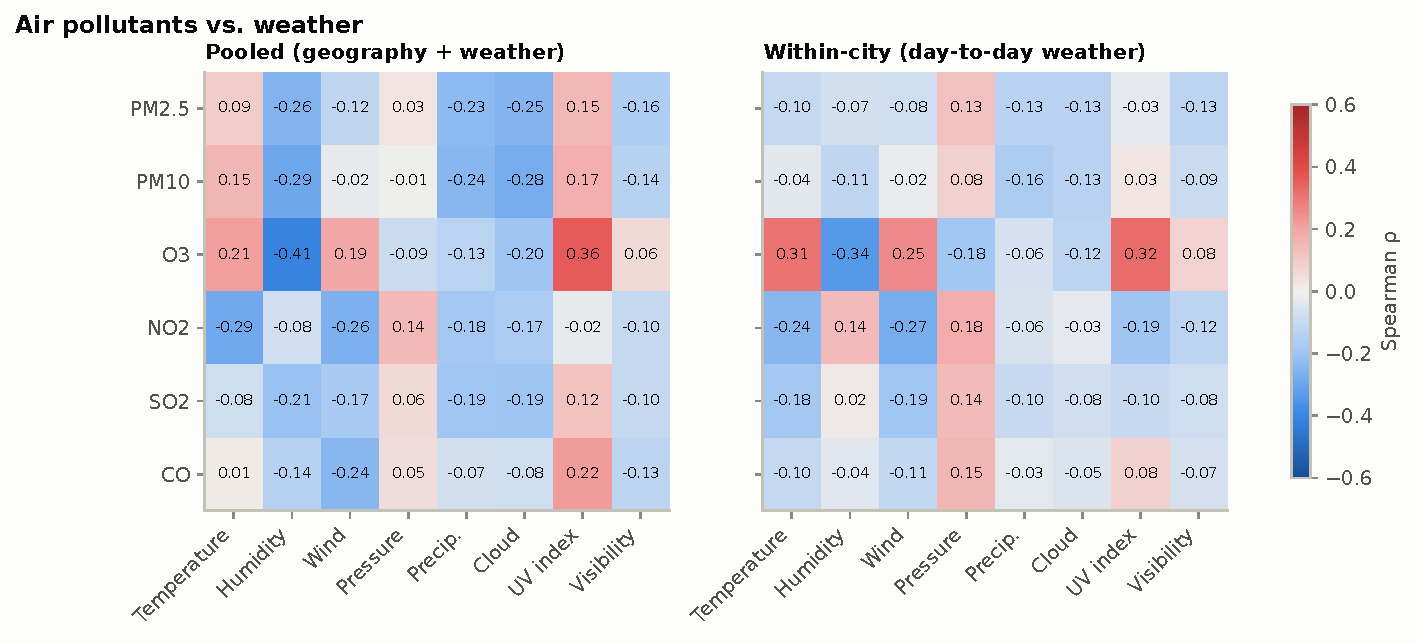
\includegraphics[width=\linewidth]{analyses/airquality_weather_correlation}
\caption{Air pollutants against weather: pooled (left) and within-city (right) Spearman correlations.}\label{fig:aqcorr}
\end{figure}
\begin{figure}[H]\centering
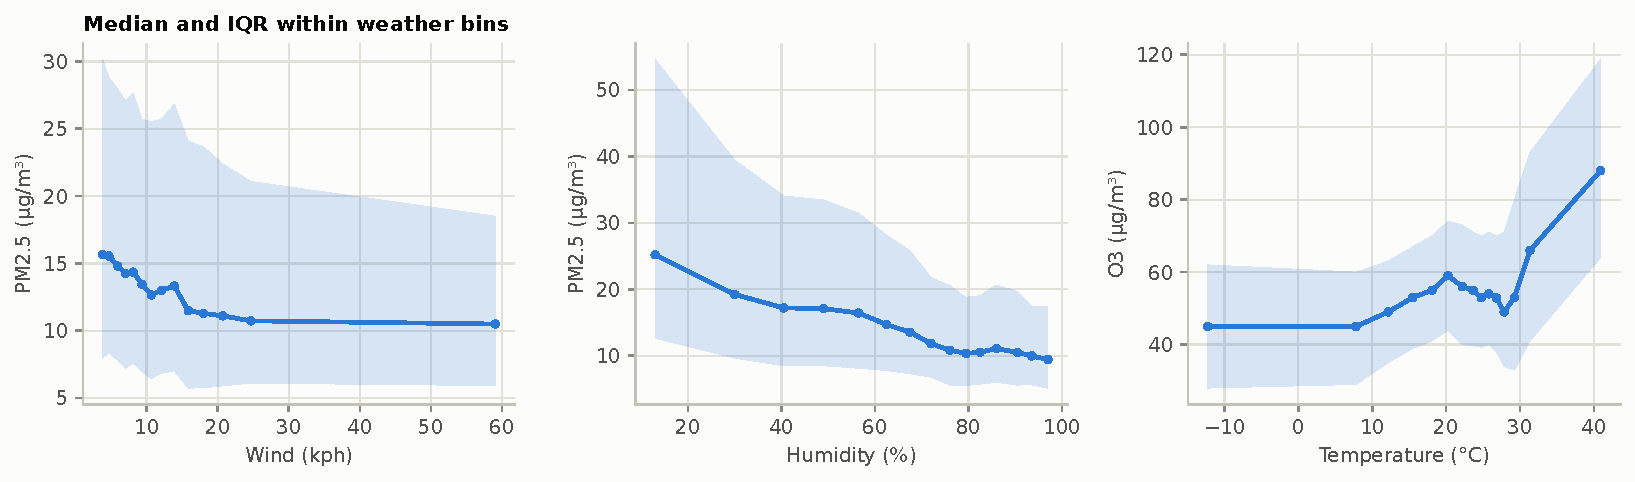
\includegraphics[width=\linewidth]{analyses/airquality_response_curves}
\caption{Pollutant response within weather bins (median and IQR).}
\end{figure}
\begin{figure}[H]\centering
\begin{subfigure}{0.49\linewidth}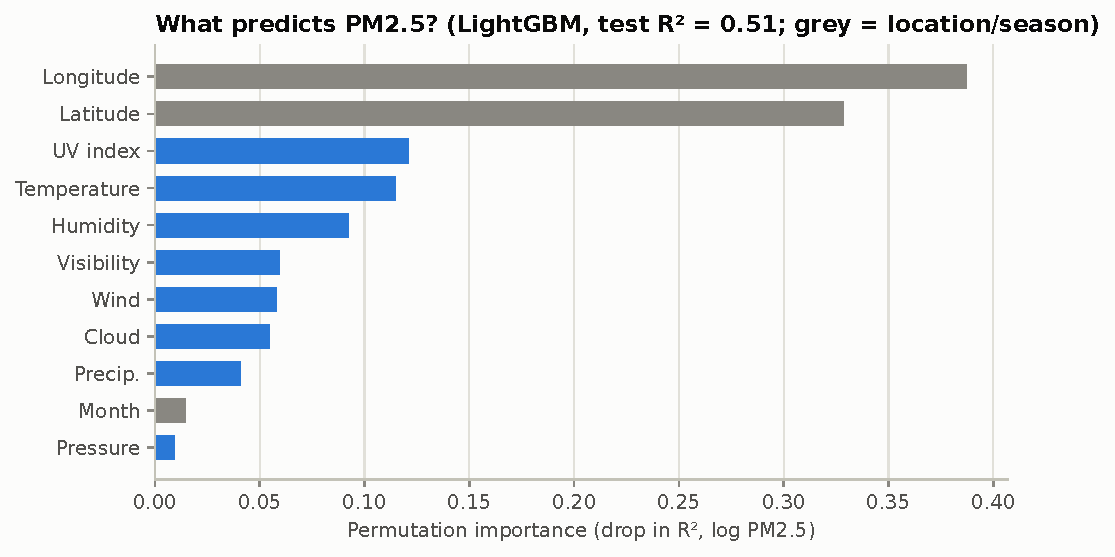
\includegraphics[width=\linewidth]{analyses/airquality_pm25_drivers}\caption{Drivers of PM2.5}\label{fig:pmdrivers}\end{subfigure}
\begin{subfigure}{0.49\linewidth}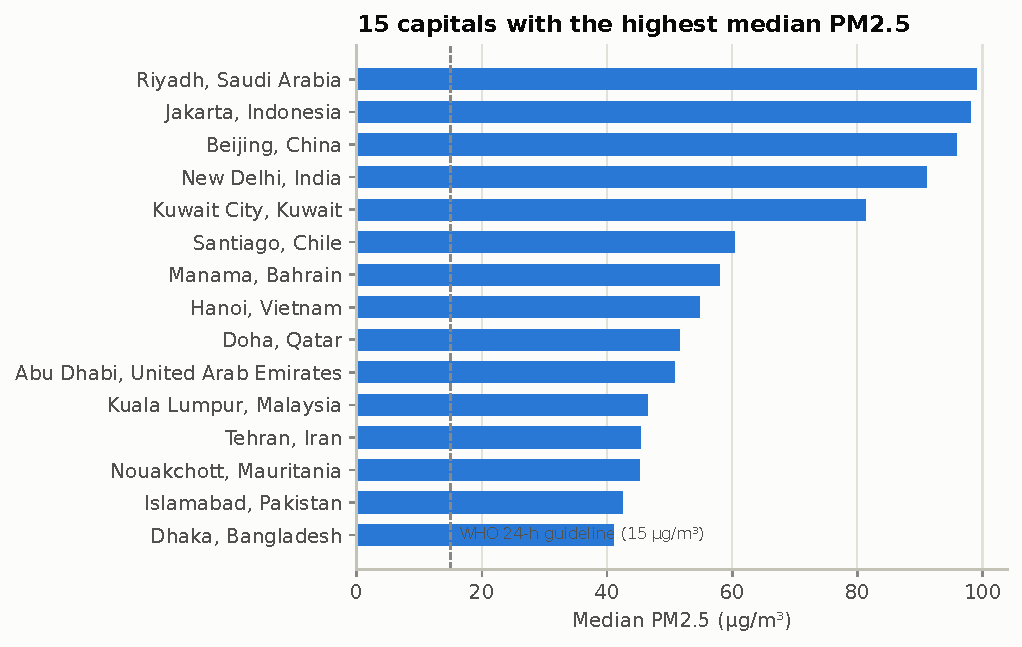
\includegraphics[width=\linewidth]{analyses/airquality_top_pm25}\caption{Most polluted capitals}\end{subfigure}
\caption{Air-quality drivers and hotspots.}
\end{figure}
\begin{figure}[H]\centering
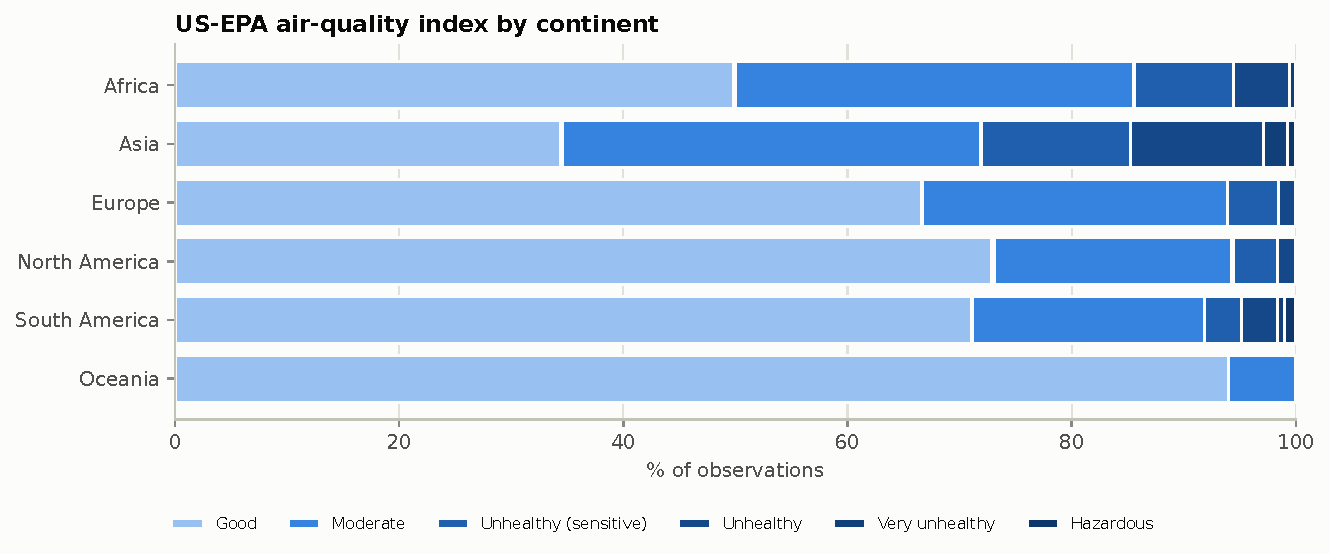
\includegraphics[width=0.9\linewidth]{analyses/airquality_epa_by_continent}
\caption{US-EPA air-quality index categories by continent.}
\end{figure}

\subsection{Feature importance}
Feature importance for the LightGBM next-day model is assessed four ways: split \textbf{gain},
\textbf{permutation} (increase in test RMSE), \textbf{mean $|$SHAP$|$} (TreeExplainer) and \textbf{mutual
information}. All four agree that persistence dominates: current temperature first, then its 3-, 7- and 14-day
rolling means and the feels-like temperature (Table~\ref{tab:feature_importance}). Gain and SHAP rankings
correlate at $\rho=0.73$, and permutation and SHAP at $\rho=0.83$. Mutual information also rewards redundant
features, such as raw lags, that the trees do not need. Past the persistence block, the secondary signals are
humidity, pressure and its daily change, latitude, UV, and the diurnal snapshot-hour terms
(Figure~\ref{fig:fi2}).

\tbl{feature_importance.tex}
\begin{figure}[H]\centering
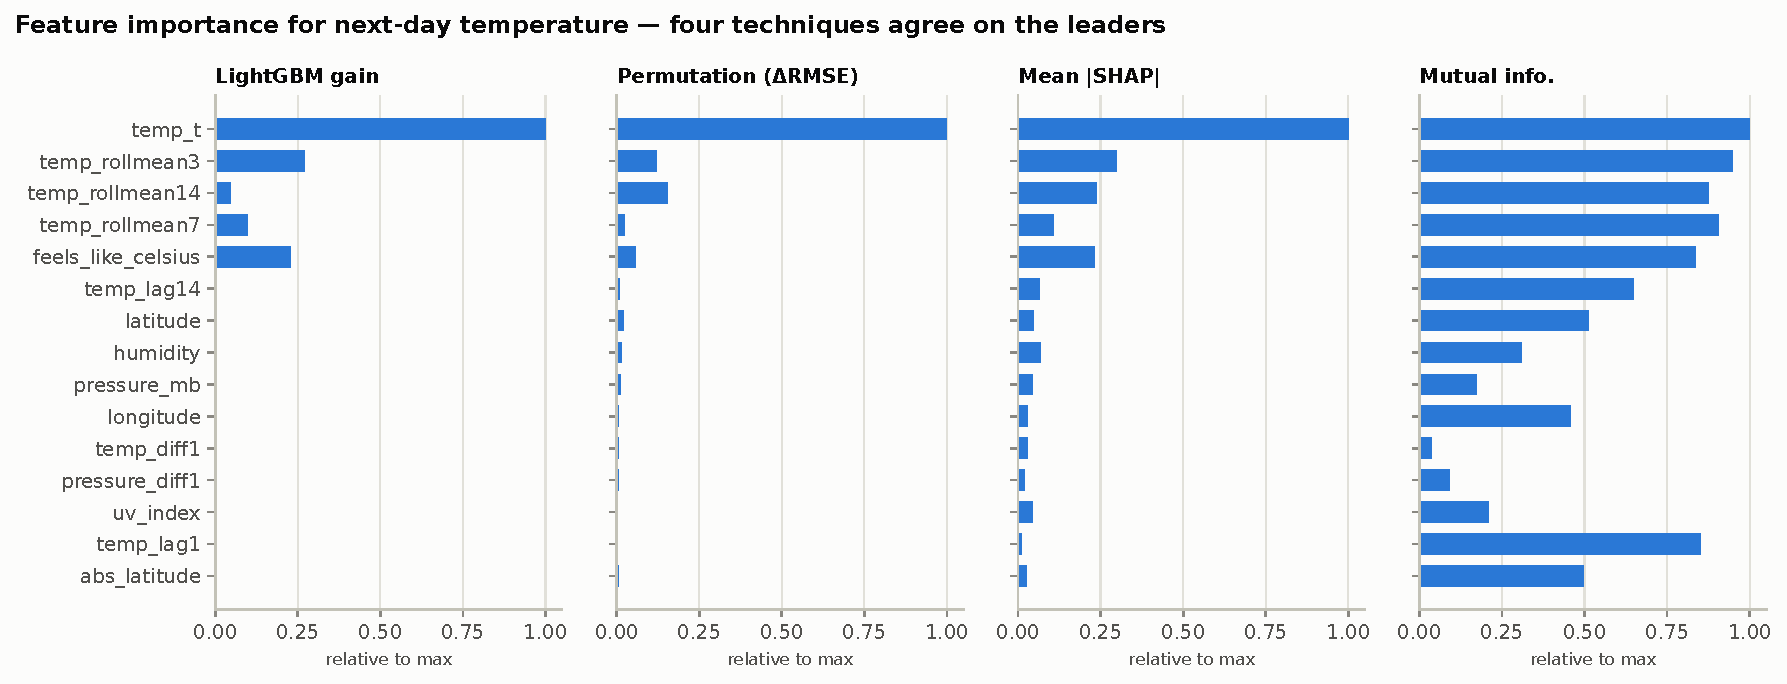
\includegraphics[width=\linewidth]{analyses/feature_importance_comparison}
\caption{Top-15 features under four importance techniques, each scaled to its maximum.}
\end{figure}
\begin{figure}[H]\centering
\begin{subfigure}{0.49\linewidth}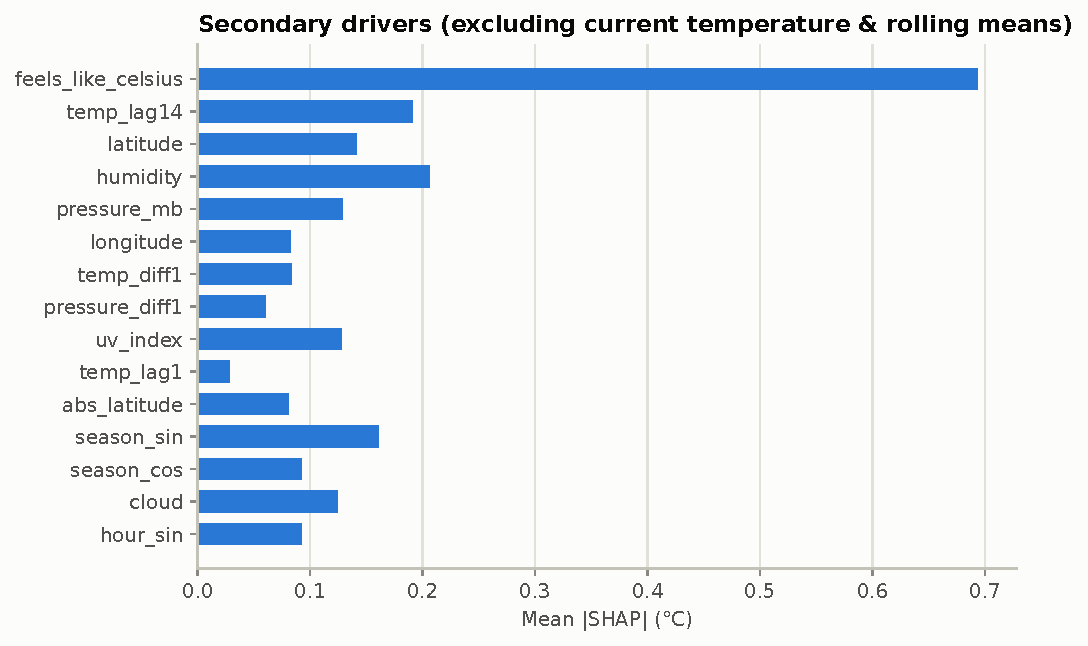
\includegraphics[width=\linewidth]{analyses/feature_importance_secondary}\caption{Secondary drivers}\label{fig:fi2}\end{subfigure}
\begin{subfigure}{0.49\linewidth}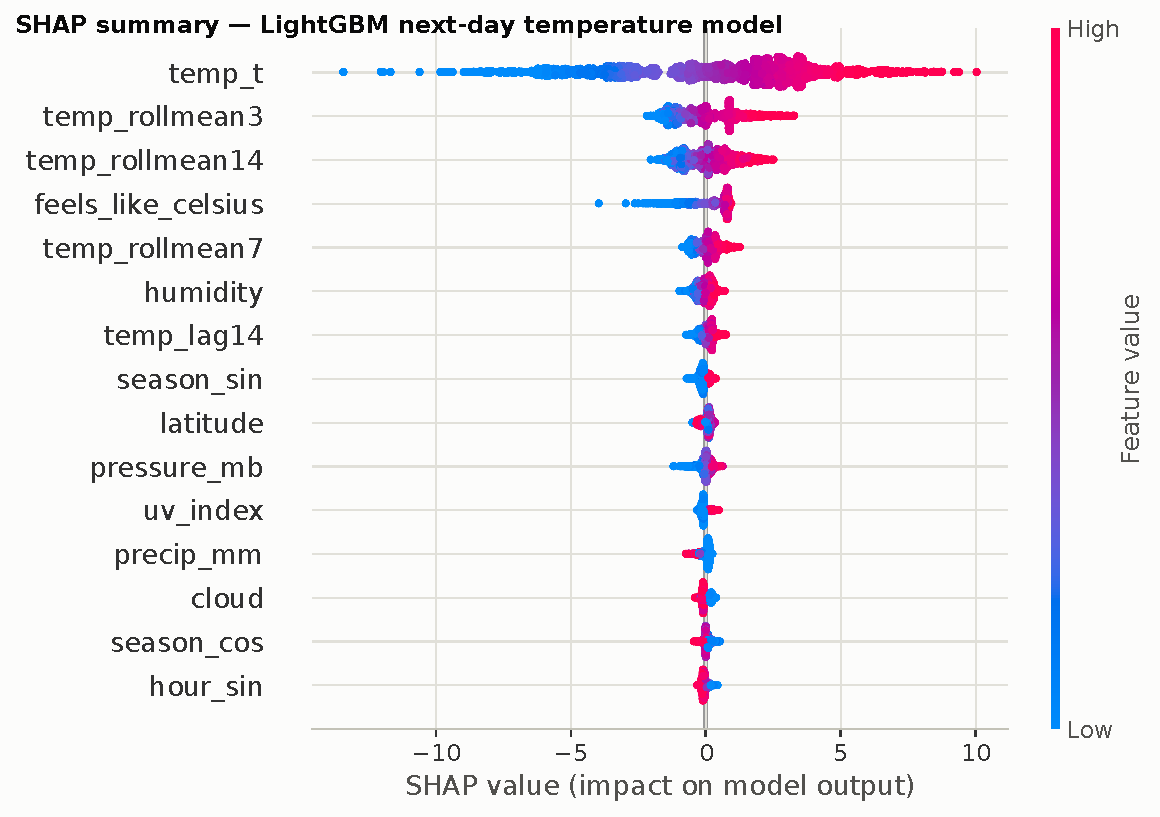
\includegraphics[width=\linewidth]{analyses/feature_importance_shap_summary}\caption{SHAP summary}\end{subfigure}
\caption{Feature importance beyond persistence, and a SHAP beeswarm.}
\end{figure}

\subsection{Spatial analysis}
Every variable is clustered in space. Moran's $I$ with 8-nearest-neighbour great-circle weights and 999
permutations gives $p=0.001$ for all four variables (Figure~\ref{fig:spatial}): temperature $I=0.68$,
humidity $0.71$, precipitation $0.54$ and PM2.5 $0.31$. PM2.5 is the least spatially structured because it
depends on local emissions. Temperature declines away from the equator, faster in the Northern Hemisphere,
where most high-latitude capitals lie (Figure~\ref{fig:latprof}). Interactive maps are produced in
\texttt{reports/maps/}: a Folium map of all capitals with pop-ups, and Plotly maps.

\begin{figure}[H]\centering
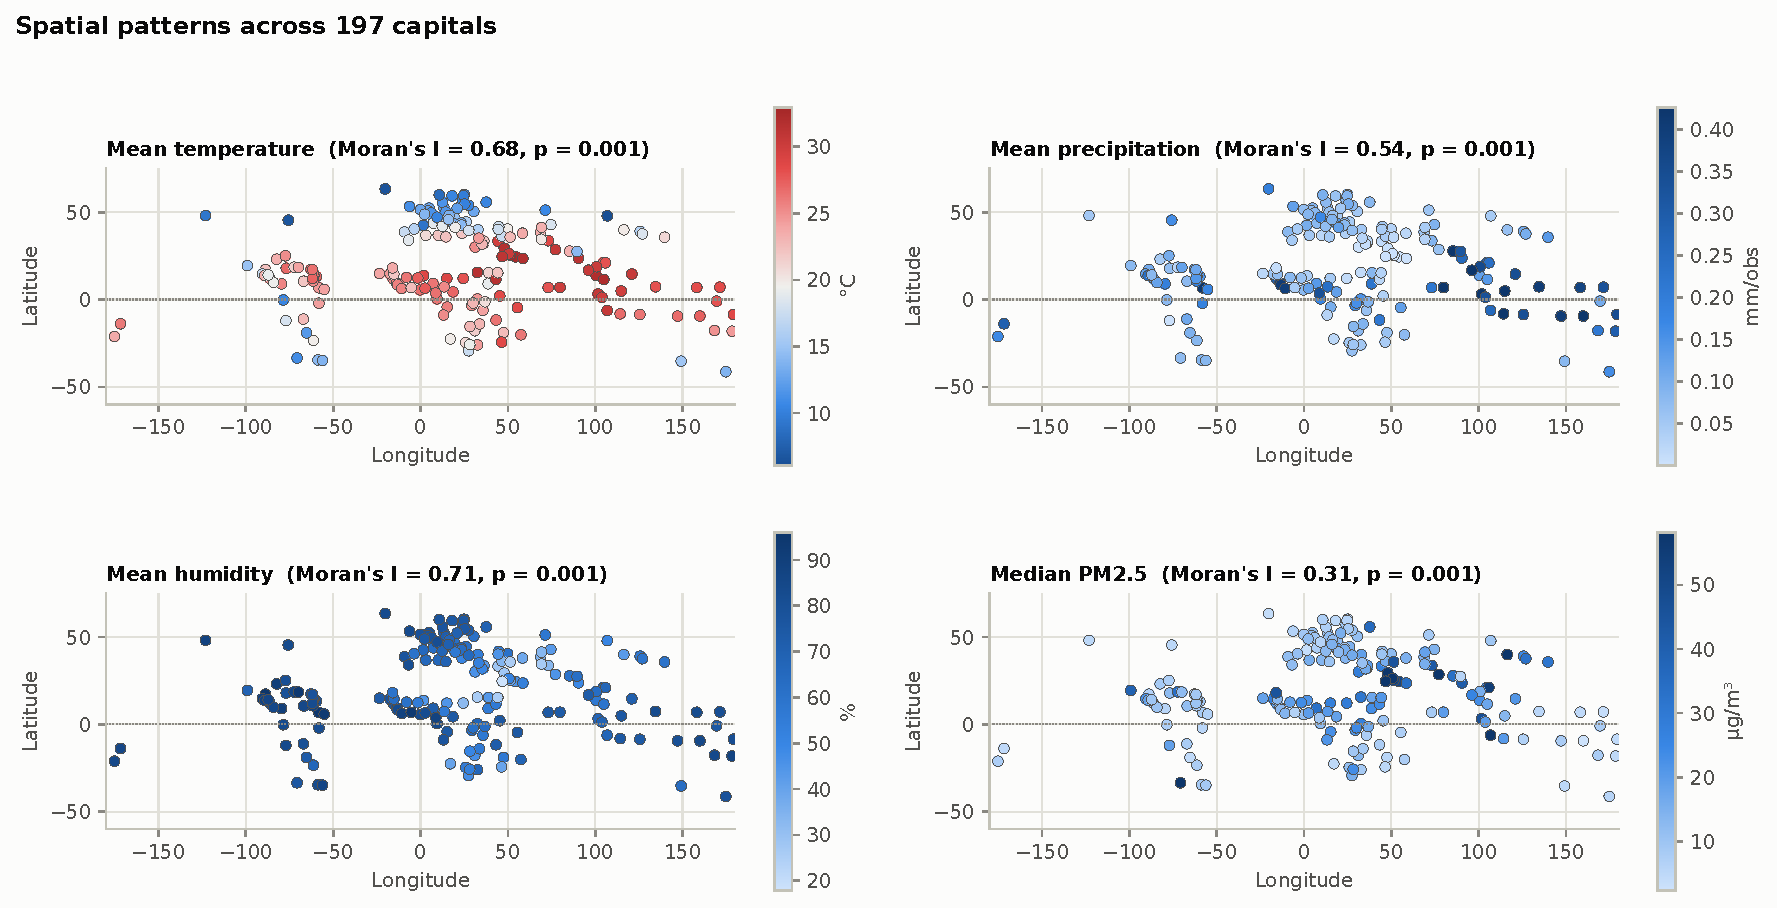
\includegraphics[width=\linewidth]{analyses/spatial_maps}
\caption{Spatial distribution of climate and air quality, with Moran's $I$.}\label{fig:spatial}
\end{figure}
\begin{figure}[H]\centering
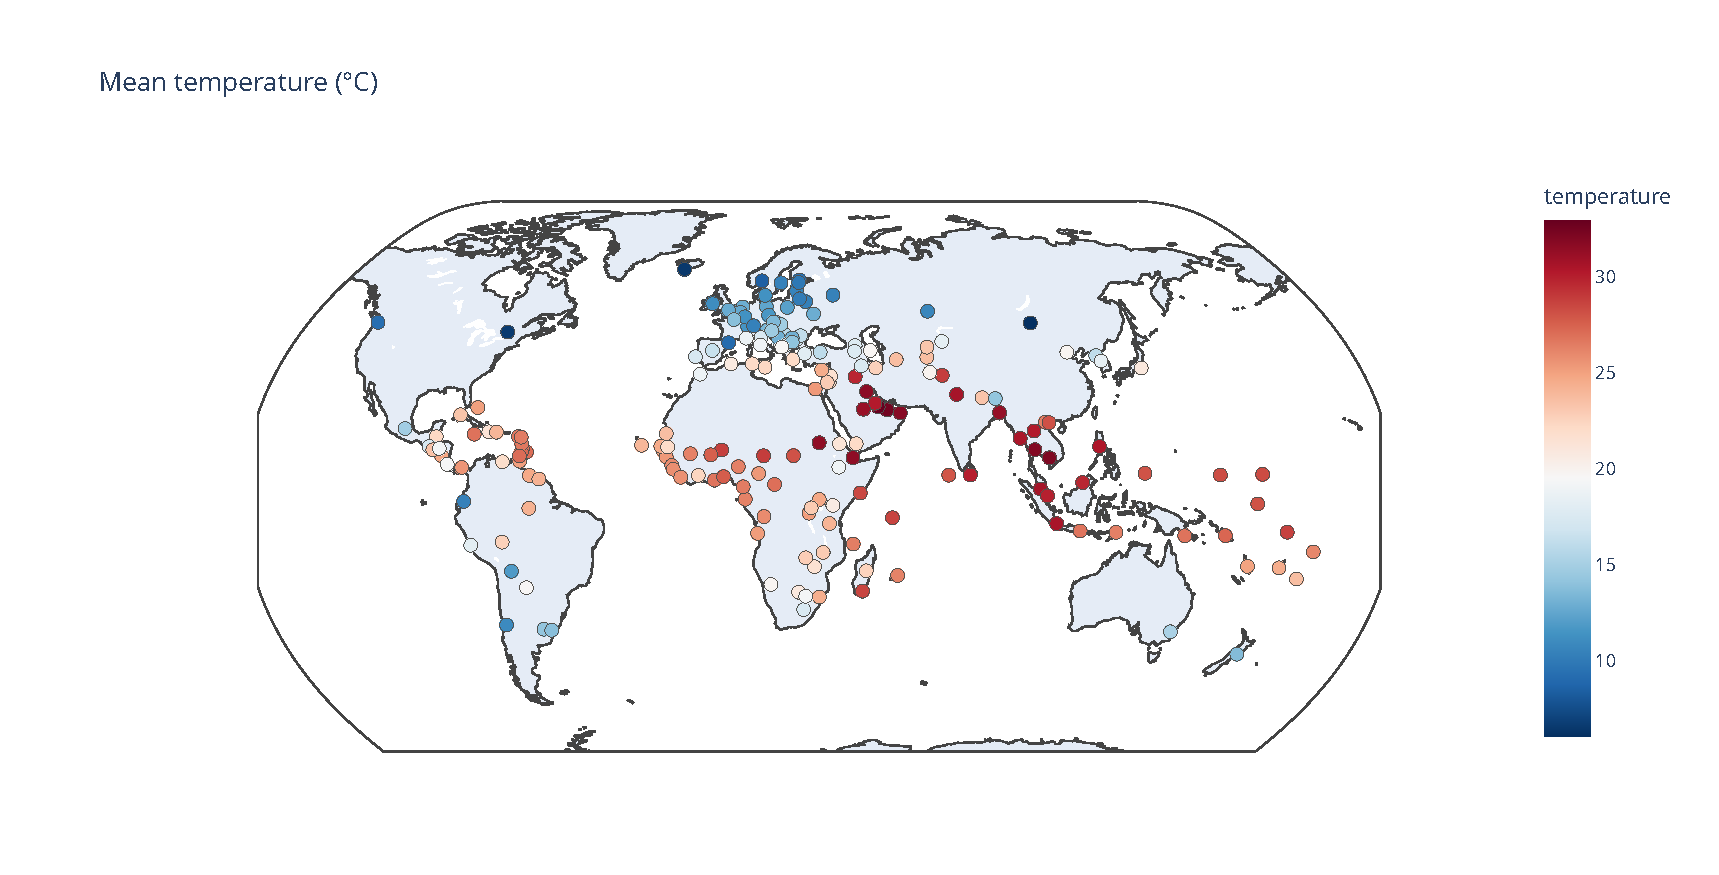
\includegraphics[width=0.85\linewidth]{analyses/geo_map_temperature}
\caption{Mean temperature of the 197 capitals (natural-earth projection).}
\end{figure}
\begin{figure}[H]\centering
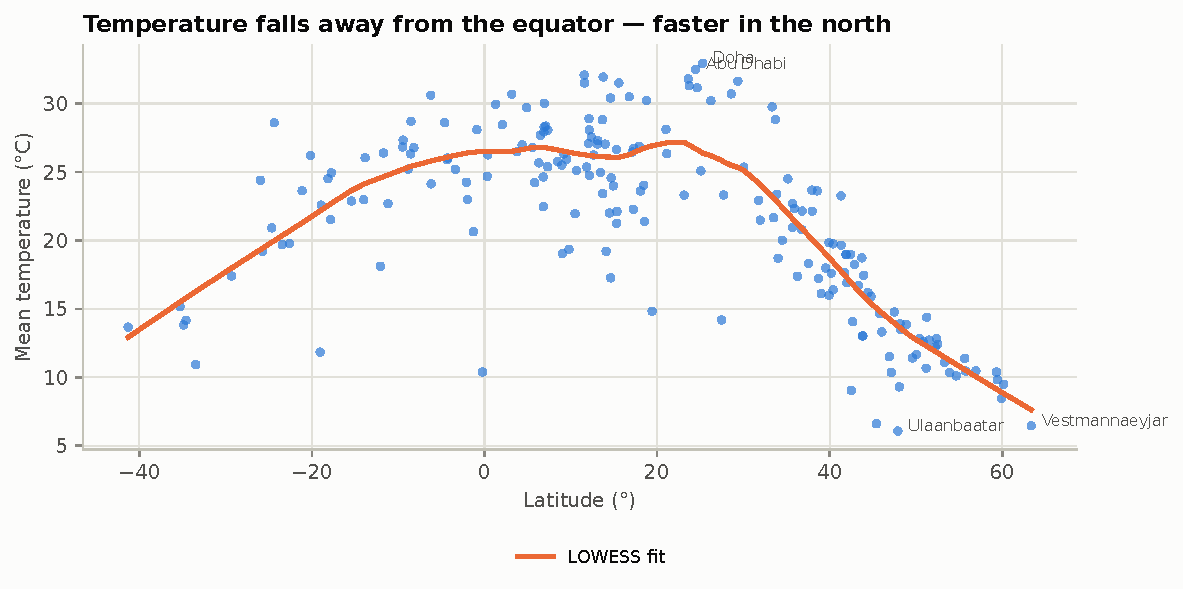
\includegraphics[width=0.85\linewidth]{analyses/spatial_latitude_profile}
\caption{Latitude profile of mean temperature with a LOWESS fit.}\label{fig:latprof}
\end{figure}

\subsection{Geographical patterns}
\tbl{continent_summary.tex}
Doha is the hottest capital in the sample (32.9\,\textdegree C mean) and Ulaanbaatar the coldest
(6.1\,\textdegree C). Asia has both the widest temperature spread and the highest median PM2.5. Europe is
cool and humid with clean air, while Africa and Oceania are warm with narrow ranges
(Figure~\ref{fig:geobox}). Per-country summaries are in \texttt{reports/tables/country\_summary.csv}.

\begin{figure}[H]\centering
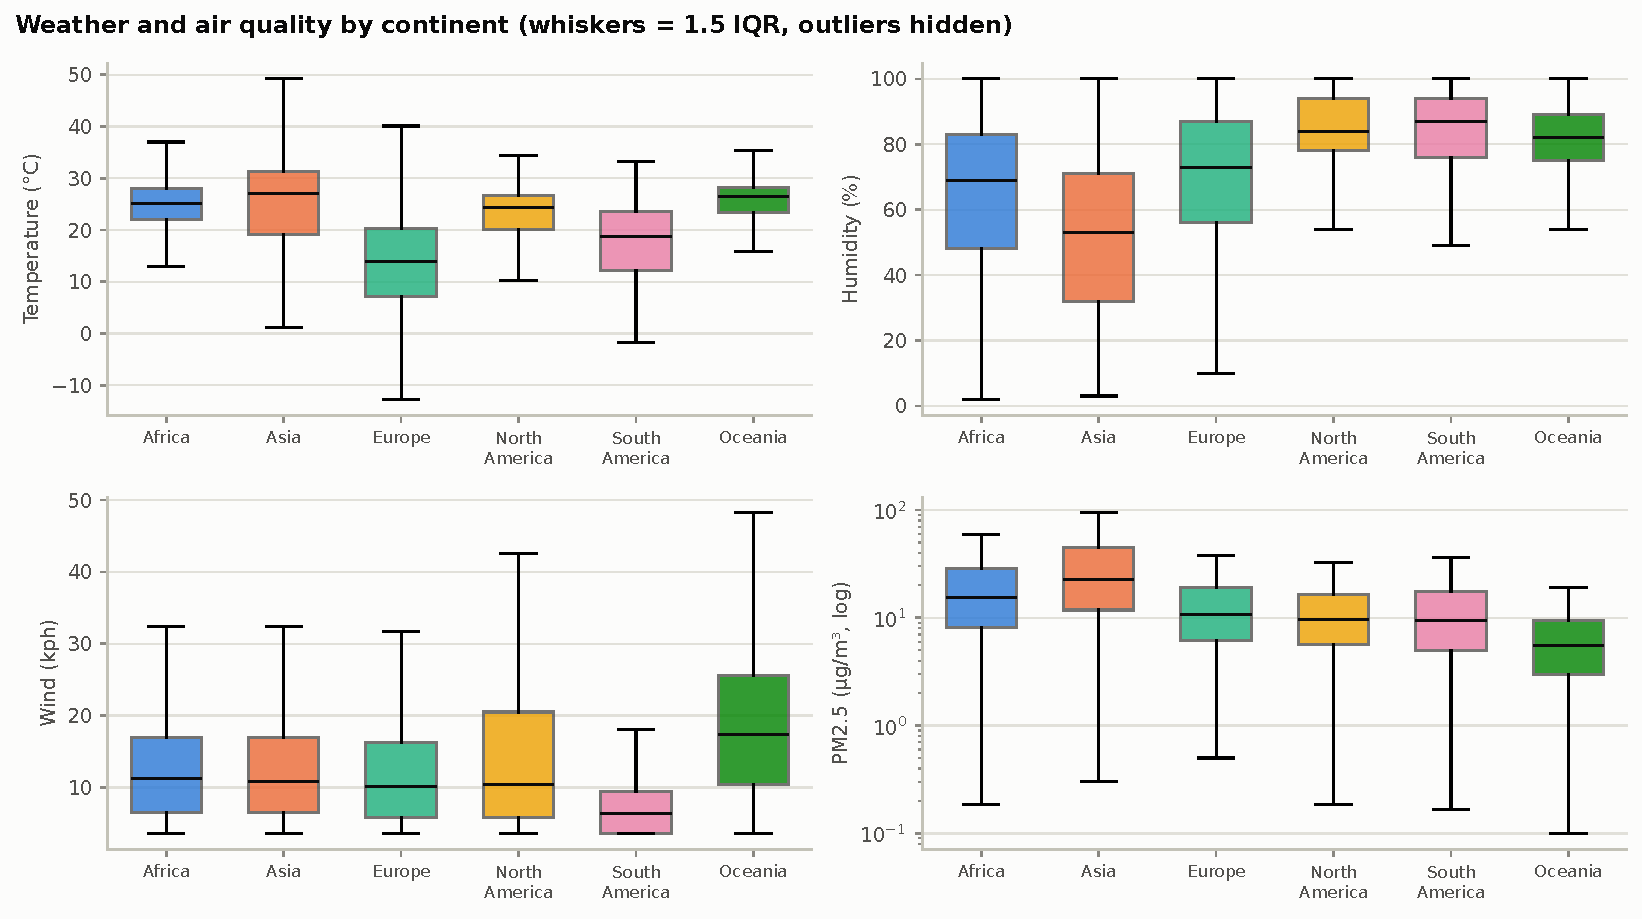
\includegraphics[width=\linewidth]{analyses/geo_continent_boxplots}
\caption{Weather and air quality by continent.}\label{fig:geobox}
\end{figure}
\begin{figure}[H]\centering
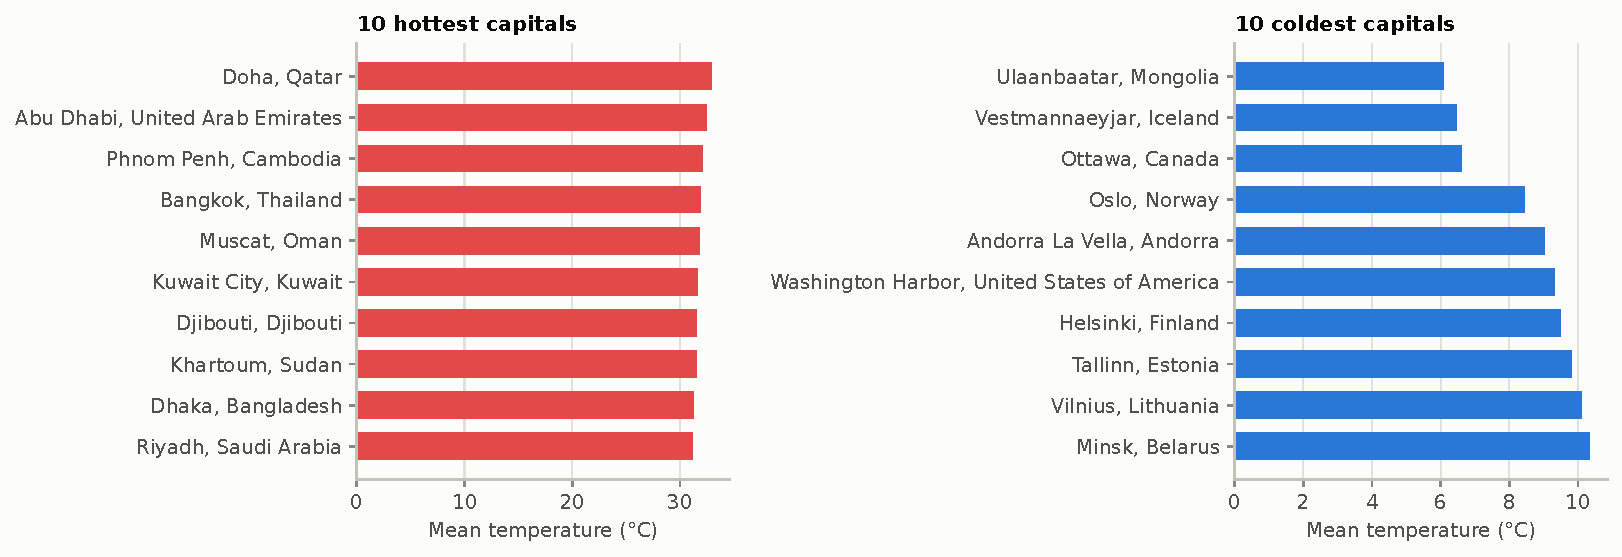
\includegraphics[width=\linewidth]{analyses/geo_hottest_coldest}
\caption{The hottest and coldest capitals by mean temperature.}
\end{figure}

\section{Key insights}
\begin{enumerate}
  \item \textbf{Check how the data was collected before fitting any trend.} The local time of the daily
        snapshot drifts from afternoon to early morning, which creates an artificial cooling of about
        1.8\,\textdegree C/yr. Correcting for it removes most of that trend and improves multi-step
        forecasts by about 40\,\%.
  \item \textbf{The source feed has failures of its own.} One whole day (17~Aug~2026) is corrupted across all
        cities. A batch-level detector catches it; a per-city outlier fence would not.
  \item \textbf{Next-day temperature is mostly persistence.} The stacked ensemble improves RMSE on persistence
        by 12\,\% (1.84 against 2.09\,\textdegree C), and ensembles beat every single model.
  \item \textbf{Global seasonal trends are highly predictable.} The global mean is forecast 60 days ahead
        with an RMSE of about 0.35\,\textdegree C.
  \item \textbf{Air quality is mostly local.} Ozone follows sunshine and heat. PM2.5 is driven mostly by
        location, and weather explains only a small share of its day-to-day variation.
  \item \textbf{Climate has strong spatial structure.} Temperature and humidity have Moran's $I$ near 0.7,
        and the size of the annual cycle is largely set by latitude.
\end{enumerate}

\paragraph{Limitations.} The record covers about 2.4 years, so long-term climate trends cannot be estimated.
There is one instantaneous snapshot per day, not a daily mean or extreme. Some locations are geocoding
homonyms. Pollutant values come from a model-based feed.

\paragraph{Next steps.}
\begin{itemize}
  \item Aggregate the 15-minute API data, or re-weight observations by local hour.
  \item Add multi-horizon direct models for days 1--7.
  \item Add probabilistic forecasts (quantile LightGBM).
  \item Add ERA5 reanalysis as a long-term baseline.
\end{itemize}

\section{Reproducibility}
\begin{itemize}
  \item \textbf{Environment}: \texttt{uv} (\texttt{pyproject.toml} and \texttt{uv.lock}), Python 3.12;
        formatting and linting with \texttt{black} and \texttt{ruff}, enforced by a pre-commit hook.
  \item \textbf{Configuration}: every setting (paths, MLflow, data source, cleaning thresholds, features,
        split, hyper-parameters) is in \nolinkurl{.env}. It is loaded into a typed pydantic settings model with
        nested sections and validation, built once by a cached \texttt{get\_settings()}
        (\nolinkurl{src/weather/utils/config.py}). Environment variables override the file.
  \item \textbf{Pipeline}: \texttt{uv run dvc repro} rebuilds every artefact. Every stage depends on
        \nolinkurl{.env}, and \texttt{dvc metrics diff} compares experiments.
  \item \textbf{Data versioning}: raw and processed data and model binaries are DVC-tracked and pushed to a
        DVC remote. Figures, tables and metrics are committed to git.
  \item \textbf{Experiment tracking}: \texttt{uv run mlflow ui --backend-store-uri sqlite:///mlflow.db}
        shows one run per stage, nested runs per model, artefacts, and registered models.
  \item \textbf{Tests}: \texttt{uv run pytest}. The suite covers cleaning rules, corrupted-batch detection,
        alignment of features and targets, strict time ordering of the split (no leakage), and the metrics.
\end{itemize}

\end{document}
